\documentclass[a4paper]{article}
\usepackage[utf8]{inputenc}
\usepackage[spanish, es-tabla]{babel}

\usepackage[a4paper, footnotesep = 1cm, width=18cm, left=2cm, top=2.5cm, height=25cm, textwidth=18cm, textheight=25cm]{geometry}
%\geometry{showframe}

\usepackage{tikz}
\usepackage{amsmath}
\usepackage{amsfonts}
\usepackage{amssymb}
\usepackage{float}
\usepackage{graphicx}
\usepackage{caption}
\usepackage{subcaption}
\usepackage{multicol}
\usepackage{multirow}
\setlength{\doublerulesep}{\arrayrulewidth}
\usepackage{xcolor}

\usepackage{hyperref}
\hypersetup{
    colorlinks=true,
    linkcolor=blue,
    filecolor=magenta,      
    urlcolor=blue,
    citecolor=blue,    
}

\newcommand{\quotes}[1]{``#1''}
\usepackage{array}
\newcolumntype{C}[1]{>{\centering\let\newline\\\arraybackslash\hspace{0pt}}m{#1}}
\usepackage[american]{circuitikz}
\usepackage{fancyhdr}
\usepackage{units} 

\pagestyle{fancy}
\fancyhf{}
\lhead{22.13 Electrónica III}
\rhead{Mechoulam, Lambertucci, Martorell, Londero}
\rfoot{\center \thepage}
\usepackage{tikz}
\usetikzlibrary{matrix,calc}

%isolated term
%#1 - Optional. Space between node and grouping line. Default=0
%#2 - node
%#3 - filling color
\newcommand{\implicantsol}[3][0]{
    \draw[rounded corners=3pt, fill=#3, opacity=0.3] ($(#2.north west)+(135:#1)$) rectangle ($(#2.south east)+(-45:#1)$);
    }


%internal group
%#1 - Optional. Space between node and grouping line. Default=0
%#2 - top left node
%#3 - bottom right node
%#4 - filling color
\newcommand{\implicant}[4][0]{
    \draw[rounded corners=3pt, fill=#4, opacity=0.3] ($(#2.north west)+(135:#1)$) rectangle ($(#3.south east)+(-45:#1)$);
    }

%group lateral borders
%#1 - Optional. Space between node and grouping line. Default=0
%#2 - top left node
%#3 - bottom right node
%#4 - filling color
\newcommand{\implicantcostats}[4][0]{
    \draw[rounded corners=3pt, fill=#4, opacity=0.3] ($(rf.east |- #2.north)+(90:#1)$)-| ($(#2.east)+(0:#1)$) |- ($(rf.east |- #3.south)+(-90:#1)$);
    \draw[rounded corners=3pt, fill=#4, opacity=0.3] ($(cf.west |- #2.north)+(90:#1)$) -| ($(#3.west)+(180:#1)$) |- ($(cf.west |- #3.south)+(-90:#1)$);
}

%group top-bottom borders
%#1 - Optional. Space between node and grouping line. Default=0
%#2 - top left node
%#3 - bottom right node
%#4 - filling color
\newcommand{\implicantdaltbaix}[4][0]{
    \draw[rounded corners=3pt, fill=#4, opacity=0.3] ($(cf.south -| #2.west)+(180:#1)$) |- ($(#2.south)+(-90:#1)$) -| ($(cf.south -| #3.east)+(0:#1)$);
    \draw[rounded corners=3pt, fill=#4, opacity=0.3] ($(rf.north -| #2.west)+(180:#1)$) |- ($(#3.north)+(90:#1)$) -| ($(rf.north -| #3.east)+(0:#1)$);
}

%group corners
%#1 - Optional. Space between node and grouping line. Default=0
%#2 - filling color
\newcommand{\implicantcantons}[2][0]{
    \draw[rounded corners=3pt, opacity=.3] ($(rf.east |- 0.south)+(-90:#1)$) -| ($(0.east |- cf.south)+(0:#1)$);
    \draw[rounded corners=3pt, opacity=.3] ($(rf.east |- 8.north)+(90:#1)$) -| ($(8.east |- rf.north)+(0:#1)$);
    \draw[rounded corners=3pt, opacity=.3] ($(cf.west |- 2.south)+(-90:#1)$) -| ($(2.west |- cf.south)+(180:#1)$);
    \draw[rounded corners=3pt, opacity=.3] ($(cf.west |- 10.north)+(90:#1)$) -| ($(10.west |- rf.north)+(180:#1)$);
    \fill[rounded corners=3pt, fill=#2, opacity=.3] ($(rf.east |- 0.south)+(-90:#1)$) -|  ($(0.east |- cf.south)+(0:#1)$) [sharp corners] ($(rf.east |- 0.south)+(-90:#1)$) |-  ($(0.east |- cf.south)+(0:#1)$) ;
    \fill[rounded corners=3pt, fill=#2, opacity=.3] ($(rf.east |- 8.north)+(90:#1)$) -| ($(8.east |- rf.north)+(0:#1)$) [sharp corners] ($(rf.east |- 8.north)+(90:#1)$) |- ($(8.east |- rf.north)+(0:#1)$) ;
    \fill[rounded corners=3pt, fill=#2, opacity=.3] ($(cf.west |- 2.south)+(-90:#1)$) -| ($(2.west |- cf.south)+(180:#1)$) [sharp corners]($(cf.west |- 2.south)+(-90:#1)$) |- ($(2.west |- cf.south)+(180:#1)$) ;
    \fill[rounded corners=3pt, fill=#2, opacity=.3] ($(cf.west |- 10.north)+(90:#1)$) -| ($(10.west |- rf.north)+(180:#1)$) [sharp corners] ($(cf.west |- 10.north)+(90:#1)$) |- ($(10.west |- rf.north)+(180:#1)$) ;
}

%Empty Karnaugh map 4x4
\newenvironment{Karnaugh}%
{
\begin{tikzpicture}[baseline=(current bounding box.north),scale=0.8]
\draw (0,0) grid (4,4);
\draw (0,4) -- node [pos=0.7,above right,anchor=south west] {ba} node [pos=0.7,below left,anchor=north east] {dc} ++(135:1);
%
\matrix (mapa) [matrix of nodes,
        column sep={0.8cm,between origins},
        row sep={0.8cm,between origins},
        every node/.style={minimum size=0.3mm},
        anchor=8.center,
        ampersand replacement=\&] at (0.5,0.5)
{
                       \& |(c00)| 00         \& |(c01)| 01         \& |(c11)| 11         \& |(c10)| 10         \& |(cf)| \phantom{00} \\
|(r00)| 00             \& |(0)|  \phantom{0} \& |(1)|  \phantom{0} \& |(3)|  \phantom{0} \& |(2)|  \phantom{0} \&                     \\
|(r01)| 01             \& |(4)|  \phantom{0} \& |(5)|  \phantom{0} \& |(7)|  \phantom{0} \& |(6)|  \phantom{0} \&                     \\
|(r11)| 11             \& |(12)| \phantom{0} \& |(13)| \phantom{0} \& |(15)| \phantom{0} \& |(14)| \phantom{0} \&                     \\
|(r10)| 10             \& |(8)|  \phantom{0} \& |(9)|  \phantom{0} \& |(11)| \phantom{0} \& |(10)| \phantom{0} \&                     \\
|(rf) | \phantom{00}   \&                    \&                    \&                    \&                    \&                     \\
};
}%
{
\end{tikzpicture}
}

%Empty Karnaugh map 2x4
\newenvironment{Karnaughvuit}%
{
\begin{tikzpicture}[baseline=(current bounding box.north),scale=0.8]
\draw (0,0) grid (4,2);
\draw (0,2) -- node [pos=0.7,above right,anchor=south west] {bc} node [pos=0.7,below left,anchor=north east] {a} ++(135:1);
%
\matrix (mapa) [matrix of nodes,
        column sep={0.8cm,between origins},
        row sep={0.8cm,between origins},
        every node/.style={minimum size=0.3mm},
        anchor=4.center,
        ampersand replacement=\&] at (0.5,0.5)
{
                      \& |(c00)| 00         \& |(c01)| 01         \& |(c11)| 11         \& |(c10)| 10         \& |(cf)| \phantom{00} \\
|(r00)| 0             \& |(0)|  \phantom{0} \& |(1)|  \phantom{0} \& |(3)|  \phantom{0} \& |(2)|  \phantom{0} \&                     \\
|(r01)| 1             \& |(4)|  \phantom{0} \& |(5)|  \phantom{0} \& |(7)|  \phantom{0} \& |(6)|  \phantom{0} \&                     \\
|(rf) | \phantom{00}  \&                    \&                    \&                    \&                    \&                     \\
};
}%
{
\end{tikzpicture}
}

%Empty Karnaugh map 2x2
\newenvironment{Karnaughquatre}%
{
\begin{tikzpicture}[baseline=(current bounding box.north),scale=0.8]
\draw (0,0) grid (2,2);
\draw (0,2) -- node [pos=0.7,above right,anchor=south west] {b} node [pos=0.7,below left,anchor=north east] {a} ++(135:1);
%
\matrix (mapa) [matrix of nodes,
        column sep={0.8cm,between origins},
        row sep={0.8cm,between origins},
        every node/.style={minimum size=0.3mm},
        anchor=2.center,
        ampersand replacement=\&] at (0.5,0.5)
{
          \& |(c00)| 0          \& |(c01)| 1  \\
|(r00)| 0 \& |(0)|  \phantom{0} \& |(1)|  \phantom{0} \\
|(r01)| 1 \& |(2)|  \phantom{0} \& |(3)|  \phantom{0} \\
};
}%
{
\end{tikzpicture}
}

%Defines 8 or 16 values (0,1,X)
\newcommand{\contingut}[1]{%
\foreach \x [count=\xi from 0]  in {#1}
     \path (\xi) node {\x};
}

%Places 1 in listed positions
\newcommand{\minterms}[1]{%
    \foreach \x in {#1}
        \path (\x) node {1};
}

%Places 0 in listed positions
\newcommand{\maxterms}[1]{%
    \foreach \x in {#1}
        \path (\x) node {0};
}

%Places X in listed positions
\newcommand{\indeterminats}[1]{%
    \foreach \x in {#1}
        \path (\x) node {X};
}

% \begin{document}
%     \begin{Karnaugh}
%         \contingut{0,0,0,0,0,0,0,0,0,0,0,0,0,0,0,0}
%        \implicant{0}{2}{red}
%        \implicant{5}{15}{purple}
%        \implicantdaltbaix[3pt]{3}{10}{blue}
%     \implicantcantons[2pt]{orange}
%        \implicantcostats{4}{14}{green}
%     \end{Karnaugh}
%     %
%     \begin{Karnaughvuit}
%        \minterms{3,4}
%         \maxterms{0,1,6,7}
%        \indeterminats{2,5}
%        \implicant{3}{2}{green}
%        \implicant{4}{5}{}
%     \end{Karnaughvuit}
%     %
%     \begin{Karnaughquatre}
%         \minterms{1,2}
%        \maxterms{0,3}
%        \implicantsol{1}{green}
%        \implicantsol{2}{red}
%     \end{Karnaughquatre}

% \end{document}
\usetikzlibrary{patterns}

% defining the new dimensions and parameters
\newlength{\hatchspread}
\newlength{\hatchthickness}
\newlength{\hatchshift}
\newcommand{\hatchcolor}{}
% declaring the keys in tikz
\tikzset{hatchspread/.code={\setlength{\hatchspread}{#1}},
         hatchthickness/.code={\setlength{\hatchthickness}{#1}},
         hatchshift/.code={\setlength{\hatchshift}{#1}},% must be >= 0
         hatchcolor/.code={\renewcommand{\hatchcolor}{#1}}}
% setting the default values
\tikzset{hatchspread=3pt,
         hatchthickness=0.4pt,
         hatchshift=0pt,% must be >= 0
         hatchcolor=black}
% declaring the pattern
\pgfdeclarepatternformonly[\hatchspread,\hatchthickness,\hatchshift,\hatchcolor]% variables
   {custom north west lines}% name
   {\pgfqpoint{\dimexpr-2\hatchthickness}{\dimexpr-2\hatchthickness}}% lower left corner
   {\pgfqpoint{\dimexpr\hatchspread+2\hatchthickness}{\dimexpr\hatchspread+2\hatchthickness}}% upper right corner
   {\pgfqpoint{\dimexpr\hatchspread}{\dimexpr\hatchspread}}% tile size
   {% shape description
    \pgfsetlinewidth{\hatchthickness}
    \pgfpathmoveto{\pgfqpoint{0pt}{\dimexpr\hatchspread+\hatchshift}}
    \pgfpathlineto{\pgfqpoint{\dimexpr\hatchspread+0.15pt+\hatchshift}{-0.15pt}}
    \ifdim \hatchshift > 0pt
      \pgfpathmoveto{\pgfqpoint{0pt}{\hatchshift}}
      \pgfpathlineto{\pgfqpoint{\dimexpr0.15pt+\hatchshift}{-0.15pt}}
    \fi
    \pgfsetstrokecolor{\hatchcolor}
%    \pgfsetdash{{1pt}{1pt}}{0pt}% dashing cannot work correctly in all situation this way
    \pgfusepath{stroke}
   }

\begin{document}

%%%%%%%%%%%%%%%%%%%%%%%%%
%		Caratula		%
%%%%%%%%%%%%%%%%%%%%%%%%%

\begin{titlepage}
\newcommand{\HRule}{\rule{\linewidth}{0.5mm}}
\center
\mbox{\textsc{\LARGE \bfseries {Instituto Tecnológico de Buenos Aires}}}\\[1.5cm]
\textsc{\Large 22.13 Electrónica III}\\[0.5cm]


\HRule \\[0.6cm]
{ \Huge \bfseries Trabajo práctico N$^{\circ}$2}\\[0.4cm] 
\HRule \\[1.5cm]


{\large

\emph{Grupo 3}\\
\vspace{3px}

\begin{tabular}{lr} 	
\textsc{Mechoulam}, Alan  &  58438\\
\textsc{Lambertucci}, Guido Enrique  & 58009 \\
\textsc{Martorell}, Ariel  & 56209 \\
\textsc{Londero Bonaparte}, Tomás Guillermo  & 58150 \\
\end{tabular}

\vspace{20px}

\emph{Profesores}\\
\vspace{3px}
\textsc{Dewald}, Kevin\\
\textsc{Wundes}, Pablo Enrique \\
\textsc{Aguirre}, Miguel Pablo \\	

\vspace{100px}

\begin{tabular}{ll}

Presentado: & 17/10/19\\

\end{tabular}

}

\vfill

\end{titlepage}


%%%%%%%%%%%%%%%%%%%%%
%		Indice		%
%%%%%%%%%%%%%%%%%%%%%

\tableofcontents
\newpage

%%%%%%%%%%%%%%%%%%%%%
%		Informe		%
%%%%%%%%%%%%%%%%%%%%%

\section{Ejercicio 1}
	%\documentclass[a4paper]{article}
%\usepackage[utf8]{inputenc}
%\usepackage[spanish, es-tabla]{babel}
%\usepackage[table,xcdraw]{xcolor}
%\usepackage{amsmath}
%\usepackage{amsfonts}
%\usepackage{amssymb}
%
%\usepackage{float}
%\usepackage{graphicx}
%
%\usepackage{caption}
%\usepackage{subcaption}
%\captionsetup{compatibility=false}
%
%\usepackage{multirow}
%\setlength{\doublerulesep}{\arrayrulewidth}
%
%\newcommand{\quotes}[1]{``#1''}
%\newcommand\underrel[2]{\mathrel{\mathop{#2}\limits_{#1}}}
%
%\usepackage{array}
%\newcolumntype{C}[1]{>{\centering\let\newline\\\arraybackslash\hspace{0pt}}m{#1}}
%
%\usepackage[american]{circuitikz}
%\usepackage{xcolor}
%\usepackage{fancyhdr}
%
%\newlength{\stockheight}
%\usepackage{hyperref}
%
%\hypersetup{
%    colorlinks=true,
%    linkcolor=blue,
%    filecolor=magenta,      
%    urlcolor=blue,
%    citecolor=blue,    
%}
%
%\urlstyle{same}
%
%\usepackage{units} 
%\pagestyle{fancy}
%\fancyhf{}
%
%\rfoot{Página \thepage}
%
%\begin{document}

\subsection{Introducción}
En esta sección se implementó una compuerta \textbf{NOT} utilizando diversas tecnologías, siendo estas TTL (Transistor-Transistor-Logic), RTL (Resistor-Transistor-Logic) mediante transistores BJT (Bipolar Junction Transistor) y finalmente una variación de RTL utilizando un transistor MOSFET (Metal Oxide Semiconductor Field Efect Transistor).
\subsection{Comparación tecnologías.}
Usaremos dos tipos de transistores, siendo estos BJT y MOSFET.
\begin{itemize}
\item Los BJT son controlados por corriente, mientras que los MOS son controlados por tensión.
\item Los BJT tienen una respuesta mas veloz ante un cambio en su modo de funcionamiento\footnote{Saturación y corte} que los MOS dado a que poseen una menor capacidad.
\item Los transistores MOS tienen una mayor estabilidad frente a la temperatura que los BJT.	
\item Los transistores BJT cuentan con una corriente de polarización de base que los MOS no tienen ($I_g =0$).
\item La impedancia de entrada de los MOS es mucho mayor que la de los BJT.
\end{itemize}

\subsection{Circuitos Propuestos.}
Los circuitos propuestos son los siguientes:

\begin{figure}[H]
    \centering
    \begin{subfigure}[H]{0.3\textwidth}
        \centering
		\begin{circuitikz}
		\draw
		%%%%%%%%%%%%%%%%%%%%%
		%Figuras
		%%%%%%%%%%%%%%%%%%%%%
		node[npn](np1){}
		%%%%%%%%%%%%%%%%%%%%%
		%np1
		%%%%%%%%%%%%%%%%%%%%%
		(np1.E) to ++(0,-0.5)
			node[ground]{}
		(np1.B) to[R] ++ (-1.5,0)
			to[short,-o]++(-0.5,0)
			node[label=west:$V_{In}$]{}
		(np1.C) to [R,](0,2)
			to[short,-o]++(0,0.5)
			node[label= north:$V_{cc}$]{}
		(np1.C) to [short,-o]++(0.5,0)
			node[label = east:$V_{Out}$]{}
		;
		\end{circuitikz}

        \caption{RTL}
    \end{subfigure}%
    ~ 
      \begin{subfigure}[H]{0.3\textwidth}
        \centering
	\begin{circuitikz}
	\draw
	%%%%%%%%%%%%%%%%%%%%%
	%Figuras
	%%%%%%%%%%%%%%%%%%%%%
	node[nigfete](monch){}
	%%%%%%%%%%%%%%%%%%%%%
	%monch
	%%%%%%%%%%%%%%%%%%%%%
	(monch.S) to ++(0,-0.5)
		node[ground]{}
	(monch.G) to[R] ++ (-1.5,0)
		to[short,-o]++(-0.5,0)
		node[label=west:$V_{In}$]{}
	(monch.D) to [R,](0,2)
		to[short,-o]++(0,0.5)
		node[label= north:$V_{cc}$]{}
	(monch.D) to [short,-o]++(0.5,0)
		node[label = east:$V_{Out}$]{}
	;
	\end{circuitikz}
    \caption{RTL-MOS}
    \end{subfigure}%
    ~
    \begin{subfigure}[H]{0.39\textwidth}
        \centering
		\begin{circuitikz}
		\draw
		%%%%%%%%%%%%%%%%%%%%%
		%Figuras
		%%%%%%%%%%%%%%%%%%%%%
		node[npn,rotate=-90](np1){}
		(np1.C) to[open] ++(2,0)
		node[npn](np2){}
		%%%%%%%%%%%%%%%%%%%%%
		%np1, np2
		%%%%%%%%%%%%%%%%%%%%%
		(np1.E) to[short,-o] ++ (-1,0)
			node[label = west:$V_{In}$]{}
		(np1.B) to[R,-o] ++ (0,2)
			node[label = north:$V_{cc}$]{}
		(np1.C) -- (np2.B)
		(np2.C) to[R,-o]++(0,2)
			node[label = north:$V_{cc}$]{}
		(np2.C) to[short,-o] ++(0.5,0)
			node[label = east:$V_{Out}$]{}
		(np2.E) to[short] ++ (0,-0.5)
		node[ground]{}	
		;
		\end{circuitikz}
        \caption{TTL}
    \end{subfigure}
    \caption{Circuitos propuestos}
\end{figure}


\subsection{Diseño PCB.}
Se implementó en un único PCB los 3 circuitos, que corresponden al siguiente esquemático:
\begin{figure}[H]	
	\centering
	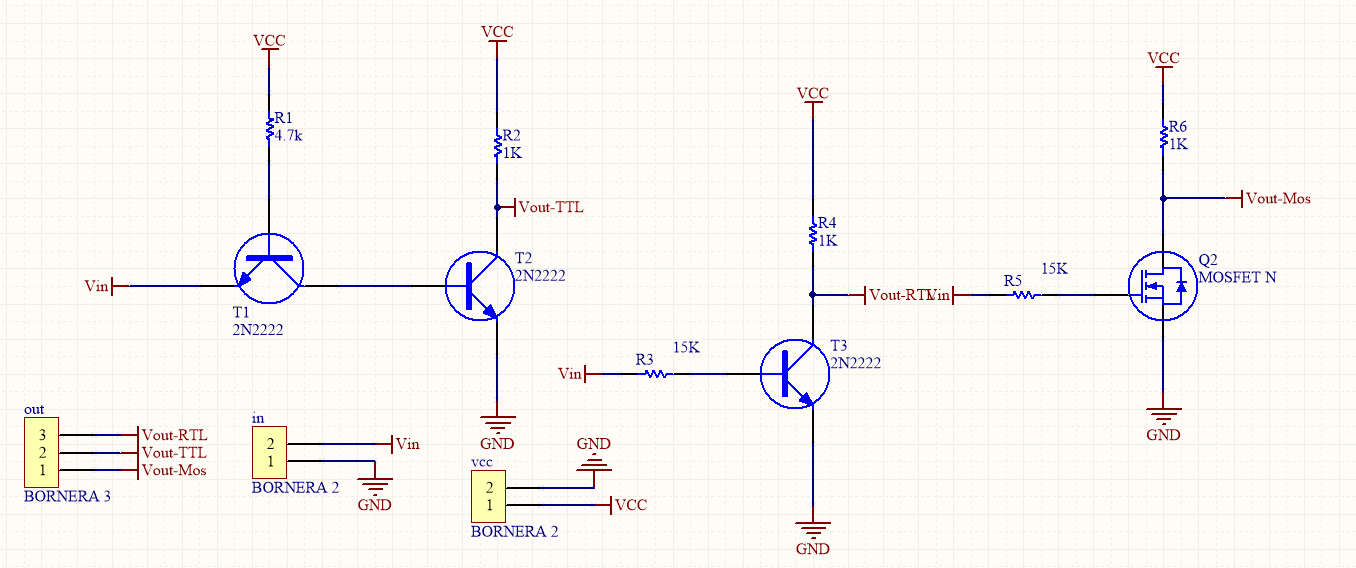
\includegraphics[width=0.5\textwidth]{Imagenes/Esquematico.PNG} \ \ \ \
	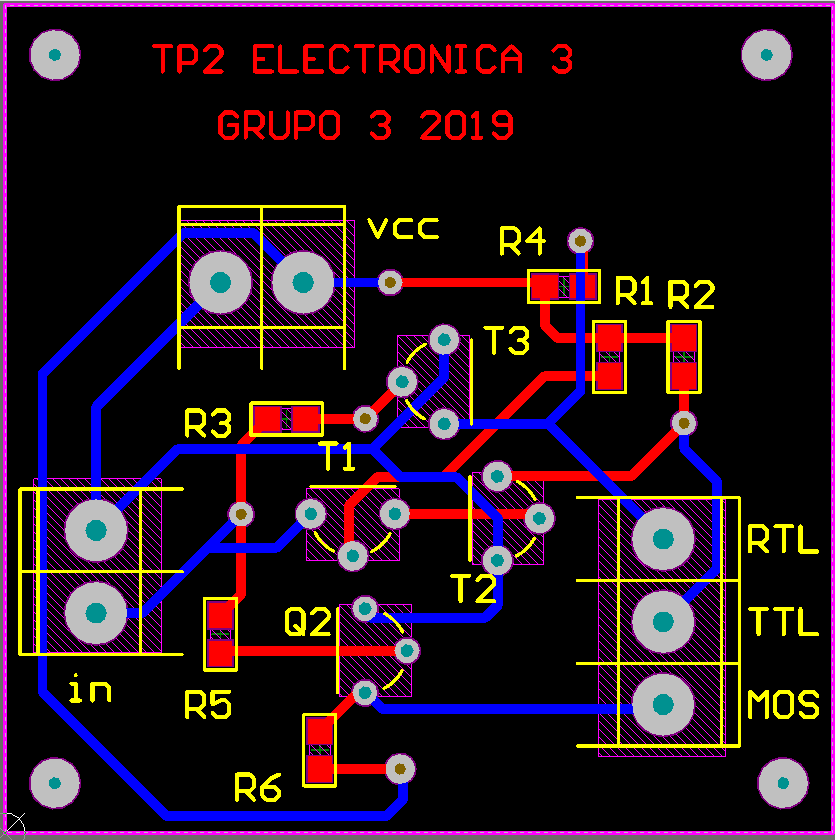
\includegraphics[width=0.3\textwidth]{Imagenes/PCB.PNG}
	\caption{Esquemático y PCB.}
	\label{fig:esquematico}
\end{figure}
%%%%%%%%%%%%%%%%%%%%%%%%%%%%%%%%%%%%%%%%%%%%%%%%%%%%%%%%

%%%%%%%%%%%%%%%%%%%%%%%%%%%%%%%%%%%%%%%%%%%%%%%%%%%%%%%%

\subsection{Observables de interés.}
\label{sec:Obs}
Se seleccionaron como observables de interés los siguientes parámetros:
\begin{enumerate}
\item \label{VIH} High-level input voltage 
\item \label{VIL} Low-level input voltage
\item \label{VOH}High-level output voltage
\item \label{VOL} Low-level output voltage
\item \label{NM}Noise Margin
\item \label{PHL}Popagation delay High to Low
\item \label{PLH}Popagation delay Low to High
\item \label{THL}Transition delay High to Low
\item \label{TLH}Transition delay Low to High
\item \label{MOC}Maximum output current
\end{enumerate}
Las mediciones de estos observables se realizaron de la siguiente manera. Para las mediciones de (\ref{VIH}), (\ref{VIL}), (\ref{VOH}), (\ref{VOL}) y (\ref{NM}) se utilizó una rampa la cual iba de un valor ligeramente inferior  a 0V  hasta 5 V, la razón de esto, es que dado a que se utilizó una rampa, contiene un salto en el cambio de periodos el cual contiene altas frecuencias y puede causar problemas, agregando ese pequeño tiempo en el cual la tenison es menor a 0V se alcanza a estabilizar la señal. La figura (\ref{fig:medramp}) es un ejemplo de una de las mediciones.
\begin{figure}[H]	
	\centering
	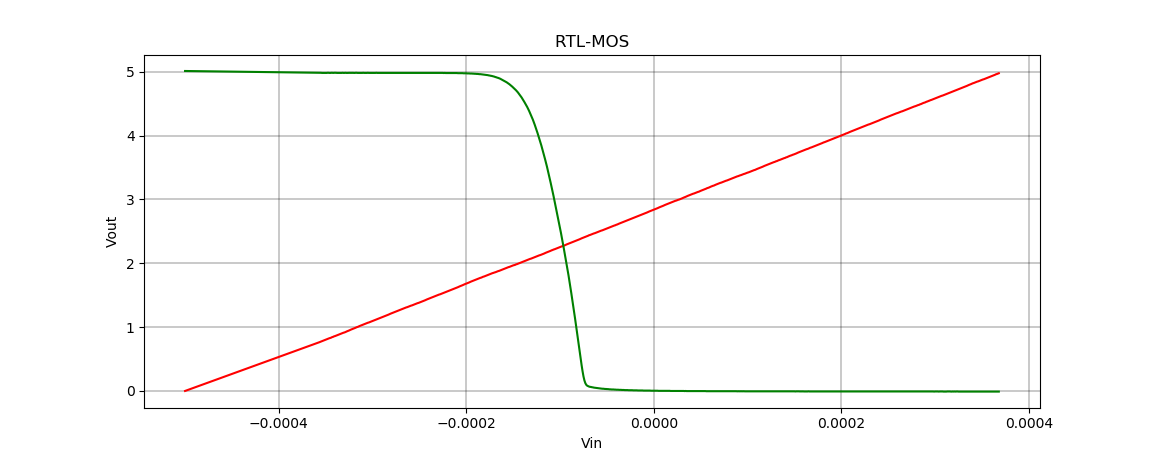
\includegraphics[width=0.9\textwidth]{Imagenes/DC-SWEEP/MedicionRampa.PNG}
	\caption{Medición niveles de tensión.}
	\label{fig:medramp}
\end{figure}
A partir de esta medición, se tomó el módulo de las señales y se graficó la señal de entrada en función de la salida, como se ve a continuación.
\begin{figure}[H]	
	\centering
	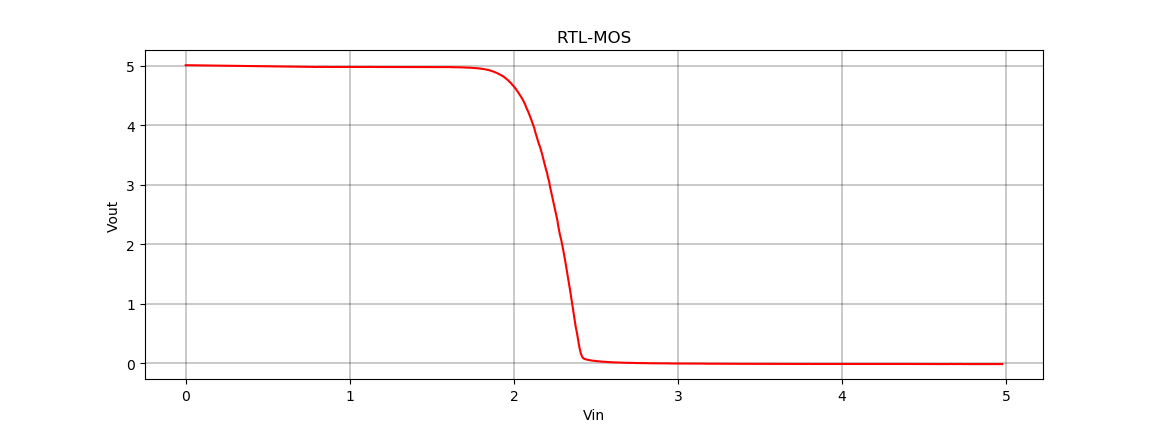
\includegraphics[width=0.9\textwidth]{Imagenes/DC-SWEEP/EntradaSalida.PNG}
	\caption{Medición entrada-salida.}
	\label{fig:medinout}
\end{figure}
finalmente a partir de esta imagen se buscó donde la pendiente es 45$^{\circ}$, de alli se obtuvo (\ref{VIH}), (\ref{VOH}), (\ref{VIL}) y (\ref{VOL}), realizando la resta de (\ref{VIH}) con (\ref{VOH}), y de (\ref{VIL}) con (\ref{VOL}) se obtienen los márgenes de ruido (\ref{NM}).

Luego para (\ref{PHL}),(\ref{PLH}),(\ref{THL}) y (\ref{TLH}) se midió la salida, con una cuadrada a la entrada como se ve en la siguiente figura:
\begin{figure}[H]	
	\centering
	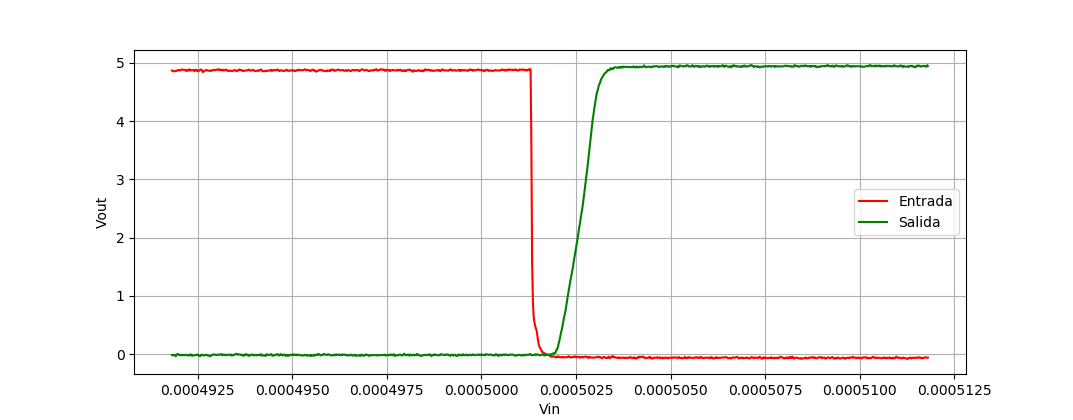
\includegraphics[width=0.9\textwidth]{Imagenes/DC-SWEEP/0t1mtl.PNG}
	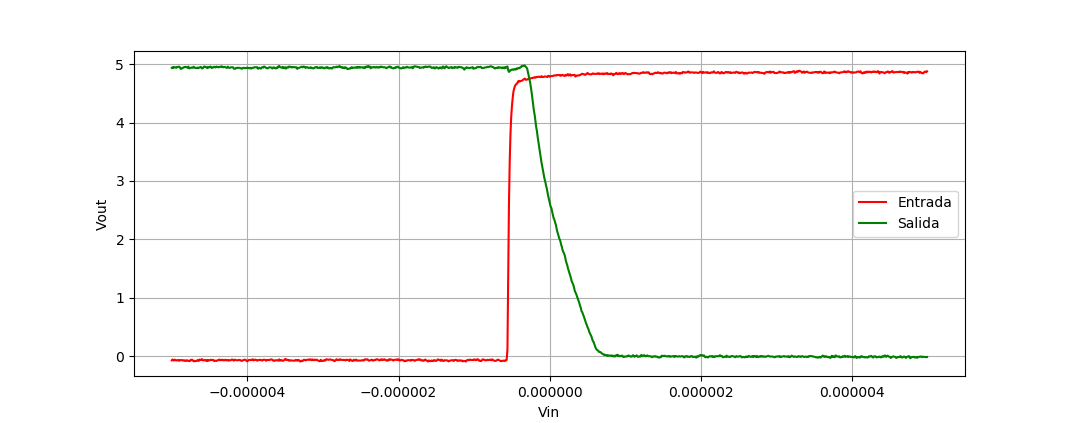
\includegraphics[width=0.9\textwidth]{Imagenes/DC-SWEEP/1t0mtl.PNG}
	\caption{Medición tiempo de propagación y transición.}
	\label{fig:MedicionTiempos}
\end{figure}
Tomando el tiempo de propagación medido al 50\% de la señal y el timpo de transición medido entre el 10 $\sim$ 90 \%. Para la medición del tiempo de propagación existe una medicion la cual dio un valor menor al tiempo de rise del osciloscopio, este resultado debe ser interpretado una cota del tiempo y no el valor exacto. 

Finalmente se colocó un trimmer de 50k$\Omega$ utilizandolo como  carga, se varió su impedancia hasta que el valor de tensión de la salida se encuentre por debajo del High Level output Voltage. A partir de este valor de tensión y la resistencia del trimmer, se obtiene la corriente máxima de salida.
\begin{figure}[H]	
	\centering
	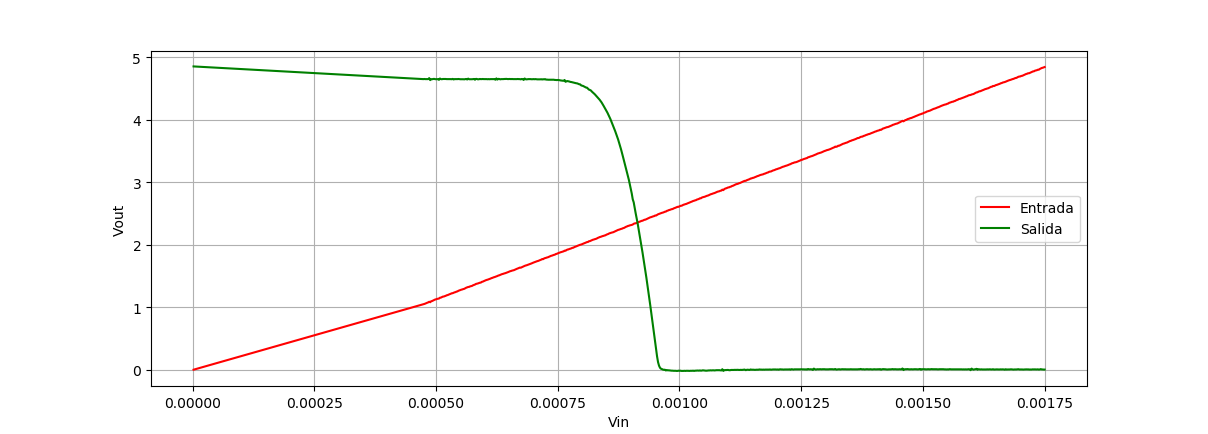
\includegraphics[width=0.9\textwidth]{Imagenes/DC-SWEEP/OutputCurrent.PNG}
	\caption{Medición corriente máxima de salida.}
	\label{fig:OutputCurrent}
\end{figure}

\subsection{Análisis de resultados.}
Para realizar una comparación entre los modelos propuestos, se utilizarán los observables de interés definidos en la sección (\ref{sec:Obs}) utlizando la siguiente tabla:
\begin{table}[H]
\centering
\begin{tabular}{c|ccc}
\hline
\multicolumn{4}{|c|}{\textit{Sin carga}}                                                                          \\ \hline
\multicolumn{1}{|c|}{\textbf{Tecnología}} & \textbf{RTL}   & \textbf{RTL-MOS} & \multicolumn{1}{c|}{\textbf{TTL}} \\ \hline
High-level input voltage                  & 864 mV         & 2.49 V           & 595 mV                            \\
Low-level input voltage                   & 454 mV         & 1.95 V           & 413 mV                            \\
High-level Output voltage                 & 4.96 V         & 4.89 V           & 4.96 V                            \\
Low-level Output voltage                  & 191 mV         & 72.1 mV          & 34.5mV                            \\
Noise Margin High                         & 4.01 V         & 2.34 V           & 4.37 V                            \\
Noise Margin Low                          & 263 mV         & 1.88 V           & 378 mV                            \\
Propagation delay High to Low             & 76.93 nS       & 569.51 nS        & 1.82 nS                           \\
Propagation delay Low to High             & 2.0489 $\mu S$ & 1.33 $\mu S$     & 535 nS                            \\
Transition delay High to Low              & 87.28 nS       & 734.4 nS         & 38.36 nS                          \\
Transition delay Low to High              & 605 nS         & 909 nS           & 307 nS                            \\
Maximum output current                    & 184.4  $\mu A$ &    217 $\mu A$              &                                  135.5$\mu A$ 	
\end{tabular}
\end{table}
%%%%%%%%%%%%%%%%%%%%%%%%%%%%%%
\begin{table}[H]
\centering
\begin{tabular}{c|ccc}
\hline
\multicolumn{4}{|c|}{\textit{Con carga}}                                                                         \\ \hline
\multicolumn{1}{|c|}{\textbf{Tecnología}} & \textbf{RTL}  & \textbf{RTL-MOS} & \multicolumn{1}{c|}{\textbf{TTL}} \\ \hline
High-level input voltage                  & 840 mV        & 2.48 V           & 627.5 mV                          \\
Low-level input voltage                   & 478.7 mV      & 2.01 V         &    490 mV                         \\
High-level Output voltage                 & 4.98 V        & 4.86 V          & 4.95 V                            \\
Low-level Output voltage                  & 278 mV        & 151 mV           & 72 mV                             \\
Noise Margin High                         & 4.14 V        & 2.52 V           & 4.32 V                            \\
Noise Margin Low                          & 200.7 mV      & 514.9 mV         & 417.3 mV                          \\
Propagation delay High to Low             & 260.7 nS      & 625.7 nS         & 33.6 nS                           \\
Propagation delay Low to High             & 2.615 $\mu S$ & 1.652 $\mu S$    & 1.216 $\mu S$                     \\
Transition delay High to Low              & 183.817 nS    & 417.19 nS        & 73.12 nS                          \\
Transition delay Low to High              & 2.691 $\mu S$ & 2.831 $\mu S$    & 2.687 $\mu S$                     \\
Maximum output current                    &  187.2 $\mu A$             &     216 $\mu A$             &   135.2 $\mu A$                               
\end{tabular}
\end{table}
 

Las diferencias entre los parámetros para las tres tecnologías son notables,
{\begin{center}\color{red} \begin{huge}
TOMI AUXILIO \end{huge} \rule{\linewidth}{0.5mm}\end{center} }

%\end{document}
\newpage	
\section{Ejercicio 2}
%	\documentclass[a4paper]{article}
\usepackage[utf8]{inputenc}
\usepackage[spanish, es-tabla]{babel}

\usepackage[a4paper, footnotesep = 1cm, width=18cm, left=2cm, top=2.5cm, height=25cm, textwidth=18cm, textheight=25cm]{geometry}
%\geometry{showframe}

\usepackage{tikz}
\usepackage{amsmath}
\usepackage{amsfonts}
\usepackage{amssymb}
\usepackage{float}
\usepackage{graphicx}
\usepackage{caption}
\usepackage{subcaption}
\usepackage{multicol}
\usepackage{multirow}
\setlength{\doublerulesep}{\arrayrulewidth}
\usepackage{xcolor}

\usepackage{hyperref}
\hypersetup{
    colorlinks=true,
    linkcolor=blue,
    filecolor=magenta,      
    urlcolor=blue,
    citecolor=blue,    
}

\newcommand{\quotes}[1]{``#1''}
\usepackage{array}
\newcolumntype{C}[1]{>{\centering\let\newline\\\arraybackslash\hspace{0pt}}m{#1}}
\usepackage[american]{circuitikz}
\usepackage{fancyhdr}
\usepackage{units} 

\pagestyle{fancy}
\fancyhf{}
\lhead{22.13 Electrónica III}
\rhead{Mechoulam, Lambertucci, Martorell, Londero}
\rfoot{\center \thepage}
\usetikzlibrary{patterns}

% defining the new dimensions and parameters
\newlength{\hatchspread}
\newlength{\hatchthickness}
\newlength{\hatchshift}
\newcommand{\hatchcolor}{}
% declaring the keys in tikz
\tikzset{hatchspread/.code={\setlength{\hatchspread}{#1}},
         hatchthickness/.code={\setlength{\hatchthickness}{#1}},
         hatchshift/.code={\setlength{\hatchshift}{#1}},% must be >= 0
         hatchcolor/.code={\renewcommand{\hatchcolor}{#1}}}
% setting the default values
\tikzset{hatchspread=3pt,
         hatchthickness=0.4pt,
         hatchshift=0pt,% must be >= 0
         hatchcolor=black}
% declaring the pattern
\pgfdeclarepatternformonly[\hatchspread,\hatchthickness,\hatchshift,\hatchcolor]% variables
   {custom north west lines}% name
   {\pgfqpoint{\dimexpr-2\hatchthickness}{\dimexpr-2\hatchthickness}}% lower left corner
   {\pgfqpoint{\dimexpr\hatchspread+2\hatchthickness}{\dimexpr\hatchspread+2\hatchthickness}}% upper right corner
   {\pgfqpoint{\dimexpr\hatchspread}{\dimexpr\hatchspread}}% tile size
   {% shape description
    \pgfsetlinewidth{\hatchthickness}
    \pgfpathmoveto{\pgfqpoint{0pt}{\dimexpr\hatchspread+\hatchshift}}
    \pgfpathlineto{\pgfqpoint{\dimexpr\hatchspread+0.15pt+\hatchshift}{-0.15pt}}
    \ifdim \hatchshift > 0pt
      \pgfpathmoveto{\pgfqpoint{0pt}{\hatchshift}}
      \pgfpathlineto{\pgfqpoint{\dimexpr0.15pt+\hatchshift}{-0.15pt}}
    \fi
    \pgfsetstrokecolor{\hatchcolor}
%    \pgfsetdash{{1pt}{1pt}}{0pt}% dashing cannot work correctly in all situation this way
    \pgfusepath{stroke}
   }

\begin{document}
\subsection{Análisis de tecnologías}

En esta instancia del informe, se procede a comparar compuertas lógicas del tipo NOR de diversas tecnologías. Para ello se vale de las hojas de datos de las compuertas \href{http://www.ti.com/lit/ds/symlink/sn74hc02.pdf}{74HC02}, \href{http://www.ti.com/lit/ds/symlink/sn74hct02.pdf}{74HCT02} y \href{http://www.ti.com/lit/ds/symlink/sn74ls02.pdf}{74LS02}. Previo a dicho análisis, cabe detallar cada una de las tecnologías. Primero, se encuentra el 74HC02, siendo este, como su nombre lo indica, del tipo HC, cuyas siglas significan ``High-speed CMOS'', tecnología caracterizada por ser de baja potencia y alta velocidad. Luego se encuentra el 74HCT02, siendo HCT una variación de las HC. Esta denominación proviene de las mismas siglas previamente mencionadas, solo que ademas posee compatibilidad con la tecnología conocida como ``logica transistor–transistor'' (TTL). En otras palabras, este tipo de compuertas puede operar bajo dicho estándar de tensiones, tanto de alimentación como de input.\footnote{``Logic family'', En.wikipedia.org, 2019. [Online]. Available: \url{https://en.wikipedia.org/wiki/Logic\_family\#HC\_logic}. [Accessed: 21- Sep- 2019].} Finalmente se encuentra el 74LS02, cuyas siglas provienen de ``Low~-power Schottky''. Los integrados de esta familia se caracterizan por estar hechos con tecnología TTL.\footnote{``Serie 7400'', Es.wikipedia.org, 2019. [Online]. Available: \url{https://es.wikipedia.org/wiki/Serie\_7400}. [Accessed: 21- Sep- 2019].} Se destaca que este último, a diferencia de los dos primeros, se caracteriza por ser fabricado mediante el uso de tecnología BJT.

Analizando las respectivas hojas de dato, se recopila información sobre los  valores aceptables de señal, tanto de entrada como de salida. Es así que se realiza la siguiente tabla:
\begin{table}[H]
\centering
\begin{tabular}{c|c|c|c|c|c|c|c|}
\cline{2-8}
                               & $\mathbf{V_{CC}}$ \textbf{[V]} & \multicolumn{2}{c|}{\textbf{74HC02}}  & \multicolumn{2}{c|}{\textbf{74HCT02}} & \multicolumn{2}{c|}{\textbf{74LS02}} \\ \cline{3-8} 
                               &              & \textbf{Min. [V]} & \textbf{Max. [V]} & \textbf{Min. [V]} & \textbf{Max. [V]} & \textbf{Min. [V]} & \textbf{Max. [V]}	\\ \hline
\multicolumn{1}{|c|}{}         & 2            & 1.9           & -            & -             & -            & -          & -            \\  
\multicolumn{1}{|c|}{$\mathbf{V_{OH}}$} & 4.5          & 4.4           & -            & 3.84          & -            & 2.7            & -            \\  
\multicolumn{1}{|c|}{}         & 6            & 5.9           & -            & -             & -            & -            & -            \\ \hline
\multicolumn{1}{|c|}{}         & 2            & -             & 0.1          & -             & -            & -            & -          \\
\multicolumn{1}{|c|}{$\mathbf{V_{OL}}$} & 4.5          & -             & 0.1          & -             & 0.33         & -            & 0.5            \\
\multicolumn{1}{|c|}{}         & 6            & -             & 0.1          & -             & -            & -            & -            \\ \hline
\multicolumn{1}{|c|}{}         & 2            & 1.5           & -            & -             & -            & -            & -            \\ 
\multicolumn{1}{|c|}{$\mathbf{V_{IH}}$}  & 4.5          & 3.15          & -            & 2             & -            & 2            & -            \\ 
\multicolumn{1}{|c|}{}         & 6            & 4.2           & -            & -             & -            & -            & -            \\ \hline
\multicolumn{1}{|c|}{}         & 2            & -             & 0.5          & -             & -            & -            & -            \\ 
\multicolumn{1}{|c|}{$\mathbf{V_{IL}}$} & 4.5          & -             & 1.35         & -             & 0.8          & -            & 0.8          \\ 
\multicolumn{1}{|c|}{}         & 6            & -             & 1.8          & -             & -            & -            & -            \\ \hline
\end{tabular}
\centering
\caption{Tabla de valores de entrada y salida.}
\label{tabla:vinout}
\end{table}

Con la información que se ha detallado, se procede a analizar el margen de ruido, tanto para los niveles altos (high), como para los bajos (low), al combinar tecnologías HC y LS, siendo este calculado de la forma
\begin{equation*}
\begin{aligned}
		NM_{High}=\ & V_{OH} - V_{IH} \\
		NM_{Low}=\ & V_{IL} - V_{OL} 
\end{aligned}
\end{equation*}

Nuevamente se decide plasmar los resultados en una tabla:
\begin{table}[H]
\centering
\begin{tabular}{|c|c|c|c|c|}
\hline
\textbf{In} & \textbf{Out} & $\mathbf{V_{CC}}$ \textbf{[V]} & $\mathbf{NM_{High}}$ \textbf{[V]} & $\mathbf{NM_{Low}} $\textbf{[V]} \\ \hline
74LS02      & 74HC02       & 4.5                            & 2.4                               & 0.7                              \\ 
74HC02      & 74LS02       & 4.5                              & -0.45                               & 0.85                                \\ \hline
\end{tabular}
\caption{Margen de ruido para combinaciones de tecnologías HC y LS.}
\label{tabla:nm}
\end{table}

Luego, se procede a representar de una forma más clara los datos obtenidos en la Tabla (\ref{tabla:vinout}) y (\ref{tabla:nm}).  

\begin{figure}[H]
\begin{center}
\begin{tikzpicture}[yscale=1]
	\node [below] at (0,0) {Out: 74HC02};
	
	\draw[-][draw=gray, line width=2mm] (0,4.4) -- (0,4.5);
	\draw[-][draw=gray, line width=2mm] (0,0) -- (0,0.1);	
	\draw[-][draw=black, very thick] (-0.2,4.4) -- (0.2,4.4);
	\draw[-][draw=black, very thick] (-0.2,0.1) -- (0.2,0.1) node[label=right:0.1 V](){};

	\draw[-][draw=black, very thick] (0,0) -- (0,4.5);
	\draw[-][draw=black, very thick] (-0.1,2.25) -- (0.1,2.25) node[label=left:2.25 V](){};
	\draw[-][draw=black, very thick] (-0.2,0) -- (0.2,0);
	\draw[-][draw=black, very thick] (-0.2,4.5) -- (0.2,4.5);
	
	\draw[-][draw=black, very thick] (-0.4,4.5) -- (-0.6,4.5);
	\draw[-][draw=black, very thick] (-0.6,4.5) -- (-0.6,4.4);
	\draw[-][draw=black, very thick] (-0.4,4.4) -- (-0.6,4.4);
	\node [left] at (-0.6,4.45) {High};
	\node [above] at (0.2,4.5) {4.5 V};
	\node [right] at (0.2,4.4) {4.4 V};
	
	\draw[-][draw=black, very thick]	 (-0.4,0) -- (-0.6,0);
	\draw[-][draw=black, very thick]	 (-0.4,0.1) -- (-0.6,0.1);
	\draw[-][draw=black, very thick]	 (-0.6,0) -- (-0.6,0.1);
	\node [left] at (-0.6,0.05) {Low};
	
	
	\node [below] at (5,0) {In: 74LS02};
	\draw[-][draw=gray, line width=2mm] (5,0) -- (5,0.8);
	\draw[-][draw=gray, line width=2mm] (5,2) -- (5,4.5);
	\draw[-][draw=black, very thick] (5.2,0.8) -- (4.8,0.8) node[label=left:0.8 V](){};
	\node [above] at (5.2,4.5) {4.5 V};
	
	\draw[-][draw=black, very thick] (5,0) -- (5,4.5);
	\draw[-][draw=black, very thick] (4.9,2.25) -- (5.1,2.25);
	\draw[-][draw=black, very thick] (4.8,0) -- (5.2,0);
	\draw[-][draw=black, very thick] (4.8,4.5) -- (5.2,4.5);
	\draw[-][draw=black, very thick] (5.4,0) -- (5.6,0);
	\draw[-][draw=black, very thick] (4.8,2) -- (5.2,2);
	\draw[-][draw=black, very thick] (5.4,0.8) -- (5.6,0.8);
	\draw[-][draw=black, very thick] (5.6,0) -- (5.6,0.8);
	\node [right] at (5.6,0.4) {Low};

	\draw[-][draw=black, very thick] (5.4,2) -- (5.6,2);
	\node [left] at (4.8,2) {2 V};	
	\draw[-][draw=black, very thick] (5.4,4.5) -- (5.6,4.5);
	\draw[-][draw=black, very thick] (5.6,2) -- (5.6,4.5);
	\node [right] at (5.6,3.25) {High};	
\end{tikzpicture}
\end{center}
\caption{Comparación de tecnologías con HC a la salida y LS a la entrada.}
\label{fig:hcls}
\end{figure}

\begin{figure}[H]
\begin{center}
\begin{tikzpicture}[yscale=1]
	\node [below] at (0,0) {Out: 74LS02};
	
	\draw[-][draw=gray, line width=2mm] (0,2.7) -- (0,4.5);
	\draw[-][draw=gray, line width=2mm] (0,0) -- (0,0.5);	
	\draw[-][draw=black, very thick] (-0.2,2.7) -- (0.2,2.7);
	\draw[-][draw=black, very thick] (-0.2,0.5) -- (0.2,0.5) node[label=right:0.5 V](){};

	\draw[-][draw=black, very thick] (0,0) -- (0,4.5);
	\draw[-][draw=black, very thick] (-0.1,2.25) -- (0.1,2.25) node[label=left:2.25 V](){};
	\draw[-][draw=black, very thick] (-0.2,0) -- (0.2,0);
	\draw[-][draw=black, very thick] (-0.2,4.5) -- (0.2,4.5);
	
	\draw[-][draw=black, very thick] (-0.4,4.5) -- (-0.6,4.5);
	\draw[-][draw=black, very thick] (-0.6,4.5) -- (-0.6,2.7);
	\draw[-][draw=black, very thick] (-0.4,2.7) -- (-0.6,2.7);
	\node [left] at (-0.6,3.6) {High};
	\node [above] at (0.2,4.5) {4.5 V};
	
	\node [right] at (0.2,2.5) {2.7 V};
	
	\draw[-][draw=black, very thick]	 (-0.4,0) -- (-0.6,0);
	\draw[-][draw=black, very thick]	 (-0.4,0.5) -- (-0.6,0.5);
	\draw[-][draw=black, very thick]	 (-0.6,0) -- (-0.6,0.5);
	\node [left] at (-0.6,0.25) {Low};
	
	
	\node [below] at (5,0) {In: 74HC02};
	\draw[-][draw=gray, line width=2mm] (5,0) -- (5,1.35);
	\draw[-][draw=gray, line width=2mm] (5,3.15) -- (5,4.5);
	\draw[-][draw=black, very thick] (5.2,1.35) -- (4.8,1.35) node[label=left:1.35 V](){};
	\node [above] at (5.2,4.5) {4.5 V};
	
	\draw[-][draw=black, very thick] (5,0) -- (5,4.5);
	\draw[-][draw=black, very thick] (4.9,2.25) -- (5.1,2.25) node[label=right:2.25 V](){};
	\draw[-][draw=black, very thick] (4.8,0) -- (5.2,0);
	\draw[-][draw=black, very thick] (4.8,4.5) -- (5.2,4.5);
	\draw[-][draw=black, very thick] (5.4,0) -- (5.6,0);
	\draw[-][draw=black, very thick] (5.2,3.15) -- (4.8,3.15);
	\draw[-][draw=black, very thick] (5.4,1.35) -- (5.6,1.35);
	\draw[-][draw=black, very thick] (5.6,0) -- (5.6,1.35);
	\node [right] at (5.6,0.675) {Low};

	\draw[-][draw=black, very thick] (5.4,3.15) -- (5.6,3.15);
		\draw[-][draw=black, very thick] (5.4,4.5) -- (5.6,4.5);
	\draw[-][draw=black, very thick] (5.6,3.15) -- (5.6,4.5);
	\node [right] at (5.6,3.825) {High};
	
	\node [left] at (4.8,3.35) {3.15 V};	
	
	\draw[pattern=custom north west lines, hatchcolor=red, hatchspread=6pt] (0,2.7) rectangle (5,3.15);	
	
\end{tikzpicture}
\end{center}
\caption{Comparación de tecnologías con LS a la salida y HC a la entrada.}
\label{fig:lshc}
\end{figure}

A la hora de conectar una compuerta con otra, es deseable que los rangos de valores validos de salida sean menores que los de entrada, ya que de esta forma se garantiza que cualquier salida sea interpretada adecuadamente por la siguiente etapa. Por consiguiente, de la Tabla (\ref{tabla:nm}) se destaca el valor negativo de $NM_{High}$ al colocar las compuertas de tecnología HC a la salida de una LS, detalle que se vuelve a observar en la Figura (\ref{fig:lshc}). Al conectar los dispositivos como se mencionó anteriormente, se pone en evidencia que existe la posibilidad de que tensiones de salida, que se consideran altas, caigan en un margen en el cual la siguiente compuerta las considera como valores imprecisos, es decir, que no actúa frente a estos. Particularmente, tensiones de salida desde $2.7 \ V$ hasta $3.15 \ V$ sin incluir, que son considerados como activos altos para la tecnología LS, no lo son para la HC. Por lo tanto, no es conveniente realizar dicha conexión, ya que se podría generar perdida de datos.

Es de esta forma que se analiza el fanout de la conexión presentada en la Figura (\ref{fig:hcls}), ya que no es conveniente llevar adelante la otra conexión presentada, debido a los motivos ya expuestos. Para ello de sebe saber cuatro factores: $I_{OH}$, $I_{OL}$, $I_{IH}$ y $I_{IL}$\footnote{``Familias Lógicas – Evolución cronológica'', Slideplayer.es, 2019. [Online]. Available: \url{https://slideplayer.es/slide/1552774/}. [Accessed: 30- Sep- 2019].}, los cuales son obtenidos de la hoja de datos. De esta forma, se calcula el fanout de la forma

\begin{equation*}
	FO = Min \left( \frac{I_{OH}}{I_{IH}}, \ \frac{I_{OL}}{I_{IL}} \right) = Min \left( \left| \frac{-4 \ mA}{20 \ \mu A} \right|, \ \left| \frac{4 \ mA}{-0.4 \ mA}\right| \right) = Min \left( 200, \ 10000 \right) = 200
\end{equation*}

\begin{center}
	\textcolor{red}{\textbf{PREGUNTAR.}}
\end{center}

\subsection{Desarrollo del circuito}

\subsection{Mediciones}

\end{document}
\newpage
\section{Ejercicio 3}
%	\documentclass[a4paper]{article}
\usepackage[utf8]{inputenc}
\usepackage[spanish, es-tabla]{babel}

\usepackage[a4paper, footnotesep = 1cm, width=18cm, left=2cm, top=2.5cm, height=25cm, textwidth=18cm, textheight=25cm]{geometry}
%\geometry{showframe}

\usepackage{tikz}
\usepackage{amsmath}
\usepackage{amsfonts}
\usepackage{amssymb}
\usepackage{float}
\usepackage{graphicx}
\usepackage{caption}
\usepackage{subcaption}
\usepackage{multicol}
\usepackage{multirow}
\setlength{\doublerulesep}{\arrayrulewidth}
\usepackage{xcolor}

\usepackage{hyperref}
\hypersetup{
    colorlinks=true,
    linkcolor=blue,
    filecolor=magenta,      
    urlcolor=blue,
    citecolor=blue,    
}

\newcommand{\quotes}[1]{``#1''}
\usepackage{array}
\newcolumntype{C}[1]{>{\centering\let\newline\\\arraybackslash\hspace{0pt}}m{#1}}
\usepackage[american]{circuitikz}
\usepackage{fancyhdr}
\usepackage{units} 

\pagestyle{fancy}
\fancyhf{}
\lhead{22.13 Electrónica III}
\rhead{Mechoulam, Lambertucci, Martorell, Londero}
\rfoot{\center \thepage}
\usepackage{tikz}
\usetikzlibrary{matrix,calc}

%isolated term
%#1 - Optional. Space between node and grouping line. Default=0
%#2 - node
%#3 - filling color
\newcommand{\implicantsol}[3][0]{
    \draw[rounded corners=3pt, fill=#3, opacity=0.3] ($(#2.north west)+(135:#1)$) rectangle ($(#2.south east)+(-45:#1)$);
    }


%internal group
%#1 - Optional. Space between node and grouping line. Default=0
%#2 - top left node
%#3 - bottom right node
%#4 - filling color
\newcommand{\implicant}[4][0]{
    \draw[rounded corners=3pt, fill=#4, opacity=0.3] ($(#2.north west)+(135:#1)$) rectangle ($(#3.south east)+(-45:#1)$);
    }

%group lateral borders
%#1 - Optional. Space between node and grouping line. Default=0
%#2 - top left node
%#3 - bottom right node
%#4 - filling color
\newcommand{\implicantcostats}[4][0]{
    \draw[rounded corners=3pt, fill=#4, opacity=0.3] ($(rf.east |- #2.north)+(90:#1)$)-| ($(#2.east)+(0:#1)$) |- ($(rf.east |- #3.south)+(-90:#1)$);
    \draw[rounded corners=3pt, fill=#4, opacity=0.3] ($(cf.west |- #2.north)+(90:#1)$) -| ($(#3.west)+(180:#1)$) |- ($(cf.west |- #3.south)+(-90:#1)$);
}

%group top-bottom borders
%#1 - Optional. Space between node and grouping line. Default=0
%#2 - top left node
%#3 - bottom right node
%#4 - filling color
\newcommand{\implicantdaltbaix}[4][0]{
    \draw[rounded corners=3pt, fill=#4, opacity=0.3] ($(cf.south -| #2.west)+(180:#1)$) |- ($(#2.south)+(-90:#1)$) -| ($(cf.south -| #3.east)+(0:#1)$);
    \draw[rounded corners=3pt, fill=#4, opacity=0.3] ($(rf.north -| #2.west)+(180:#1)$) |- ($(#3.north)+(90:#1)$) -| ($(rf.north -| #3.east)+(0:#1)$);
}

%group corners
%#1 - Optional. Space between node and grouping line. Default=0
%#2 - filling color
\newcommand{\implicantcantons}[2][0]{
    \draw[rounded corners=3pt, opacity=.3] ($(rf.east |- 0.south)+(-90:#1)$) -| ($(0.east |- cf.south)+(0:#1)$);
    \draw[rounded corners=3pt, opacity=.3] ($(rf.east |- 8.north)+(90:#1)$) -| ($(8.east |- rf.north)+(0:#1)$);
    \draw[rounded corners=3pt, opacity=.3] ($(cf.west |- 2.south)+(-90:#1)$) -| ($(2.west |- cf.south)+(180:#1)$);
    \draw[rounded corners=3pt, opacity=.3] ($(cf.west |- 10.north)+(90:#1)$) -| ($(10.west |- rf.north)+(180:#1)$);
    \fill[rounded corners=3pt, fill=#2, opacity=.3] ($(rf.east |- 0.south)+(-90:#1)$) -|  ($(0.east |- cf.south)+(0:#1)$) [sharp corners] ($(rf.east |- 0.south)+(-90:#1)$) |-  ($(0.east |- cf.south)+(0:#1)$) ;
    \fill[rounded corners=3pt, fill=#2, opacity=.3] ($(rf.east |- 8.north)+(90:#1)$) -| ($(8.east |- rf.north)+(0:#1)$) [sharp corners] ($(rf.east |- 8.north)+(90:#1)$) |- ($(8.east |- rf.north)+(0:#1)$) ;
    \fill[rounded corners=3pt, fill=#2, opacity=.3] ($(cf.west |- 2.south)+(-90:#1)$) -| ($(2.west |- cf.south)+(180:#1)$) [sharp corners]($(cf.west |- 2.south)+(-90:#1)$) |- ($(2.west |- cf.south)+(180:#1)$) ;
    \fill[rounded corners=3pt, fill=#2, opacity=.3] ($(cf.west |- 10.north)+(90:#1)$) -| ($(10.west |- rf.north)+(180:#1)$) [sharp corners] ($(cf.west |- 10.north)+(90:#1)$) |- ($(10.west |- rf.north)+(180:#1)$) ;
}

%Empty Karnaugh map 4x4
\newenvironment{Karnaugh}%
{
\begin{tikzpicture}[baseline=(current bounding box.north),scale=0.8]
\draw (0,0) grid (4,4);
\draw (0,4) -- node [pos=0.7,above right,anchor=south west] {ba} node [pos=0.7,below left,anchor=north east] {dc} ++(135:1);
%
\matrix (mapa) [matrix of nodes,
        column sep={0.8cm,between origins},
        row sep={0.8cm,between origins},
        every node/.style={minimum size=0.3mm},
        anchor=8.center,
        ampersand replacement=\&] at (0.5,0.5)
{
                       \& |(c00)| 00         \& |(c01)| 01         \& |(c11)| 11         \& |(c10)| 10         \& |(cf)| \phantom{00} \\
|(r00)| 00             \& |(0)|  \phantom{0} \& |(1)|  \phantom{0} \& |(3)|  \phantom{0} \& |(2)|  \phantom{0} \&                     \\
|(r01)| 01             \& |(4)|  \phantom{0} \& |(5)|  \phantom{0} \& |(7)|  \phantom{0} \& |(6)|  \phantom{0} \&                     \\
|(r11)| 11             \& |(12)| \phantom{0} \& |(13)| \phantom{0} \& |(15)| \phantom{0} \& |(14)| \phantom{0} \&                     \\
|(r10)| 10             \& |(8)|  \phantom{0} \& |(9)|  \phantom{0} \& |(11)| \phantom{0} \& |(10)| \phantom{0} \&                     \\
|(rf) | \phantom{00}   \&                    \&                    \&                    \&                    \&                     \\
};
}%
{
\end{tikzpicture}
}

%Empty Karnaugh map 2x4
\newenvironment{Karnaughvuit}%
{
\begin{tikzpicture}[baseline=(current bounding box.north),scale=0.8]
\draw (0,0) grid (4,2);
\draw (0,2) -- node [pos=0.7,above right,anchor=south west] {bc} node [pos=0.7,below left,anchor=north east] {a} ++(135:1);
%
\matrix (mapa) [matrix of nodes,
        column sep={0.8cm,between origins},
        row sep={0.8cm,between origins},
        every node/.style={minimum size=0.3mm},
        anchor=4.center,
        ampersand replacement=\&] at (0.5,0.5)
{
                      \& |(c00)| 00         \& |(c01)| 01         \& |(c11)| 11         \& |(c10)| 10         \& |(cf)| \phantom{00} \\
|(r00)| 0             \& |(0)|  \phantom{0} \& |(1)|  \phantom{0} \& |(3)|  \phantom{0} \& |(2)|  \phantom{0} \&                     \\
|(r01)| 1             \& |(4)|  \phantom{0} \& |(5)|  \phantom{0} \& |(7)|  \phantom{0} \& |(6)|  \phantom{0} \&                     \\
|(rf) | \phantom{00}  \&                    \&                    \&                    \&                    \&                     \\
};
}%
{
\end{tikzpicture}
}

%Empty Karnaugh map 2x2
\newenvironment{Karnaughquatre}%
{
\begin{tikzpicture}[baseline=(current bounding box.north),scale=0.8]
\draw (0,0) grid (2,2);
\draw (0,2) -- node [pos=0.7,above right,anchor=south west] {b} node [pos=0.7,below left,anchor=north east] {a} ++(135:1);
%
\matrix (mapa) [matrix of nodes,
        column sep={0.8cm,between origins},
        row sep={0.8cm,between origins},
        every node/.style={minimum size=0.3mm},
        anchor=2.center,
        ampersand replacement=\&] at (0.5,0.5)
{
          \& |(c00)| 0          \& |(c01)| 1  \\
|(r00)| 0 \& |(0)|  \phantom{0} \& |(1)|  \phantom{0} \\
|(r01)| 1 \& |(2)|  \phantom{0} \& |(3)|  \phantom{0} \\
};
}%
{
\end{tikzpicture}
}

%Defines 8 or 16 values (0,1,X)
\newcommand{\contingut}[1]{%
\foreach \x [count=\xi from 0]  in {#1}
     \path (\xi) node {\x};
}

%Places 1 in listed positions
\newcommand{\minterms}[1]{%
    \foreach \x in {#1}
        \path (\x) node {1};
}

%Places 0 in listed positions
\newcommand{\maxterms}[1]{%
    \foreach \x in {#1}
        \path (\x) node {0};
}

%Places X in listed positions
\newcommand{\indeterminats}[1]{%
    \foreach \x in {#1}
        \path (\x) node {X};
}

% \begin{document}
%     \begin{Karnaugh}
%         \contingut{0,0,0,0,0,0,0,0,0,0,0,0,0,0,0,0}
%        \implicant{0}{2}{red}
%        \implicant{5}{15}{purple}
%        \implicantdaltbaix[3pt]{3}{10}{blue}
%     \implicantcantons[2pt]{orange}
%        \implicantcostats{4}{14}{green}
%     \end{Karnaugh}
%     %
%     \begin{Karnaughvuit}
%        \minterms{3,4}
%         \maxterms{0,1,6,7}
%        \indeterminats{2,5}
%        \implicant{3}{2}{green}
%        \implicant{4}{5}{}
%     \end{Karnaughvuit}
%     %
%     \begin{Karnaughquatre}
%         \minterms{1,2}
%        \maxterms{0,3}
%        \implicantsol{1}{green}
%        \implicantsol{2}{red}
%     \end{Karnaughquatre}

% \end{document}

\begin{document}
\subsection{Introducción a riesgos estáticos}
En este punto se analiza la siguiente tabla de verdad:
\begin{table}[H]
\centering
\begin{tabular}{ccccc}
\hline
\textbf{a} & \textbf{b} & \textbf{c} &  & \textbf{Y} \\
\hline
0          & 0          & 0          &  & 0         \\
0          & 0          & 1          &  & 1         \\
0          & 1          & 0          &  & 1         \\
0          & 1          & 1          &  & 1         \\
1          & 0          & 0          &  & 0         \\
1          & 0          & 1          &  & 1         \\
1          & 1          & 0          &  & 0         \\
1          & 1          & 1          &  & 0         \\
\hline
\end{tabular}
\caption{Tabla de verdad analizada.}
\label{tabla:verdad}
\end{table}

Para ello, se vale del uso de un mapa de Karnaugh. De esta forma se encuentra su mínima expresión, la cuál se decidió expresar en minterminos.

\begin{figure}[H]
\begin{centering}
    \begin{Karnaughvuit}
        \minterms{1,2,3,5}
        \maxterms{0,4,6,7}
        
        \implicant{3}{2}{yellow}
        \implicant{1}{5}{green}   
    \end{Karnaughvuit}
\par\end{centering}
\centering
\caption{Mapa de Karnaugh de la Tabla (\ref{tabla:verdad}).}
\label{fig:karsinc}
\end{figure}

Es así, que observando la Figura (\ref{fig:karsinc}), se llega a la expresión:
\begin{equation}
	Y \left( a,b,c \right) = \bar{b} c + \bar{a} b
	\label{equ:karsinc}
\end{equation}

Una forma de representar (\ref{equ:karsinc}) se muestra en la Figura (\ref{fig:cirsinc}).

\begin{figure}[H]
\begin{center}
\begin{circuitikz}
	\node [american and port](A2){};
	\draw (A2.bin 2) node[ocirc](){};	
	\draw (A2.in 2) to[short] ++(-2,0) to[short] ++(0,4) node[circ, label=north:$b$](b){};
	\draw (A2.in 1) to[short] ++(-1,0) to[short] ++(0,3.45) node[circ, label=north:$c$](c){};
	\draw (A2) to[open] ++(0,2) node[american and port](A1){};
	\draw (A1.bin 1) node[ocirc](){};
	\draw (A1.in 2) to[short, -*] ++(-2,0);
	\draw (A1.in 1) to[short] ++(-3,0) to[short] ++(0,1.5) node[circ, label=north:$a$](a){};
	\draw (A1.out) to[short] ++(0,-0.75) node[american or port, anchor=in 1](O){};
	\draw (A2.out) |- (O.in 2);
	\draw (O.out) to[short] ++(0.5,0) node[circ, label=$y$](y){};
	\draw (A1.out) node[label=right:$\alpha$](){};
	\draw (A2.out) node[label=right:$\beta$](){};
\end{circuitikz}
\caption{Circuito posible que representa a (\ref{equ:karsinc}).}
\label{fig:cirsinc}
\end{center}
\end{figure}

Desde una perspectiva sincrónica, este circuito no presenta ningún problema, ya que las señales existentes se propagan al mismo tiempo, si ningún tipo de demora en cada compuerta. Pero desde una perspectiva asincrónica no ocurre lo mismo.

Se analiza el caso en el cual $a = 0$ y $b = c = 1$, siendo entonces $Y = 1$. Si se permite que $b$ cambie de 1 a 0, $Y$ debe seguir siendo 1. Si se considera la demora existente en la propagación de una señal a través de una compuerta, el cambio de $b$ puede llegar a ser visto en el nodo $\alpha$ antes que en el $\beta$, ya que para llegar a este último, la señal debe atravesar una compuerta más que para llegar al primero (la compuerta NOT previa a la AND). Por lo tanto, en este caso existe la posibilidad de obtener $\alpha = 0$ y $\beta = 0$, haciendo que $Y = 0$. Esto es lo que se conoce como un riesgo estático, los cuales son visibles cuando la salida debe mantenerse constante frente a un cambio de una de las variables de entrada, pero en vez de ser así, la salida varía momentáneamente para luego volver al valor debido.

\begin{figure}[H]
\begin{center}
\begin{circuitikz}
	\node [label=left:$1$](1){};
	\draw (1) to[open] ++(0.5,0) to[short] ++(1,0) to[short] ++(0,-1) to[short] ++(0.5,0) to[short] ++(0,1) to[short] ++(2,0);
	\draw (1) to[open] ++(0,-1) node[label=left:$0$](0){};
	
	\draw (0) to[open] ++(5,0) to[short] ++(1,0) to[short] ++(0,1) to[short] ++(0.5,0)to[short] ++(0,-1) to[short] ++(2,0);
\end{circuitikz}
\caption{Salida de un circuito frente a un error de riesgo estático.}
\label{fig:riesgosestaticos}
\end{center}
\end{figure}

Es posible detectar un un error potencial observando el mapa de Karnaugh, ya que en cualquier lugar que se encuentre un par de 1s adyacentes que no sean cubiertos por un grupo de minterminos, puede existir un error como el mencionado (de la misma forma ocurre con los 0s y los maxterminos). Por lo tanto, agregando algún nuevo conjunto que incluya dicho par adyacente, se evita que exista un error de transición ya que dicho conjunto se encuentra incluido en un grupo.\footnote{S. Brown and Z. Vranesic, Fundamentals of digital logic with verilog design, 3er ed. New York: McGraw-Hill, 2002.}

Por lo tanto, considerando todo lo dicho se vuelve a considerar el mapa de Karnaugh de la Tabla (\ref{tabla:verdad}), pero esta vez tomando un grupo adicional, representado en rojo:
\begin{figure}[H]
\begin{centering}
    \begin{Karnaughvuit}
        \minterms{1,2,3,5}
        \maxterms{0,4,6,7}
        
        \implicant{3}{2}{yellow}
        \implicant{1}{5}{green}
        \implicant{1}{3}{red}        
    \end{Karnaughvuit}
\par\end{centering}
\centering
\caption{Mapa de Karnaugh en un modelo asincrónico.}
\label{fig:karasinc}
\end{figure}

La consideración presentada en la Figura (\ref{fig:karasinc}) conduce a una nueva expresión, siendo esta:
\begin{equation}
	Y \left( a,b,c \right) = \bar{b} c + \bar{a} b + \bar{a} c
	\label{equ:karasinc}
\end{equation}

De la misma forma que antes, se busca representar la ecuación hallada a partir del mapa de Karnaugh mediante un circuito lógico. Esto conduce al representado en la Figura (\ref{fig:cirasinc}).

\begin{figure}[H]
\begin{center}
\begin{circuitikz}
	\node [american and port](A2){};
	\draw (A2.bin 2) node[ocirc](){};	
	\draw (A2.in 2) to[short] ++(-2,0) to[short] ++(0,4) node[circ, label=north:$b$](b){};
	\draw (A2.in 1) to[short, -*] ++(-1,0) to[short] ++(0,3.45) node[circ, label=north:$c$](c){};
	\draw (A2) to[open] ++(0,2) node[american and port](A1){};
	\draw (A1.bin 1) node[ocirc](){};
	\draw (A1.in 2) to[short, -*] ++(-2,0);
	\draw (A1.in 1) to[short, -*] ++(-3,0) to[short] ++(0,1.5) node[circ, label=north:$a$](a){};
	\draw (A2.out) to[short] ++(1,0) node[american or port, number inputs=3, anchor=in 2](O){};
	\draw (A2.out) |- (O.in 2);
	\draw (O.out) to[short] ++(0.5,0) node[circ, label=$y$](y){};
	\draw (A2) to[open] ++(0,-2) node[american and port](A3){};
	\draw (A3.bin 2) node[ocirc](){};
	\draw (a) |- (A3.in 2);
	\draw (c) |- (A3.in 1);
	\draw (A1.out) |- (O.in 1);
	\draw (A3.out) |- (O.in 3);
\end{circuitikz}
\caption{Circuito posible que representa a (\ref{equ:karasinc}).}
\label{fig:cirasinc}
\end{center}
\end{figure}

\subsection{Desarrollo del circuito}

Se implementó el circuito de la Figura (\ref{fig:cirasinc}) en un PCB. Para ello se valió del uso de las compuertas \href{http://www.ti.com/lit/ds/symlink/sn74hc04.pdf}{SN74HC04}, \href{http://www.ti.com/lit/ds/symlink/sn74hc08.pdf}{SN74HC08} y \href{http://www.ti.com/lit/ds/symlink/sn74hc32.pdf}{SN74HC32}. Para poder realizar las mediciones adecuadas, y debido a que no se contaba con una compuerta OR de tres entradas, se decidió implementar en una primera instancia lo observado en la Figura (\ref{fig:cirsinc}) (es decir, el circuito que representa a $\bar{b} c + \bar{a} b$), la cual se encuentra conectada a una bornera para poder medirla y también a otra compuerta OR, cuya segunda entrada es la resultante del termino faltante ($\bar{a} c$), la cual se encuentra conectada a otra bornera. De esta forma se puede medir tanto el circuito sin la implementación de la solución del glitch y como con dicha implementación.

\subsection{Mediciones}

Se procede a simular la situación ejemplificada previamente, es decir con  $a = 0$ y $c = 1$, alternando el valor de $b$ entre $0$ y $1$. Dicha variación se simula utilizando un generador de ondas cuadradas, el cuál oscila entre $0 \ V$ y $5 \ V$. Observando tanto la entrada como las dos salidas previamente mencionadas, se obtiene lo siguiente: 
\begin{figure}[H]
\centering
	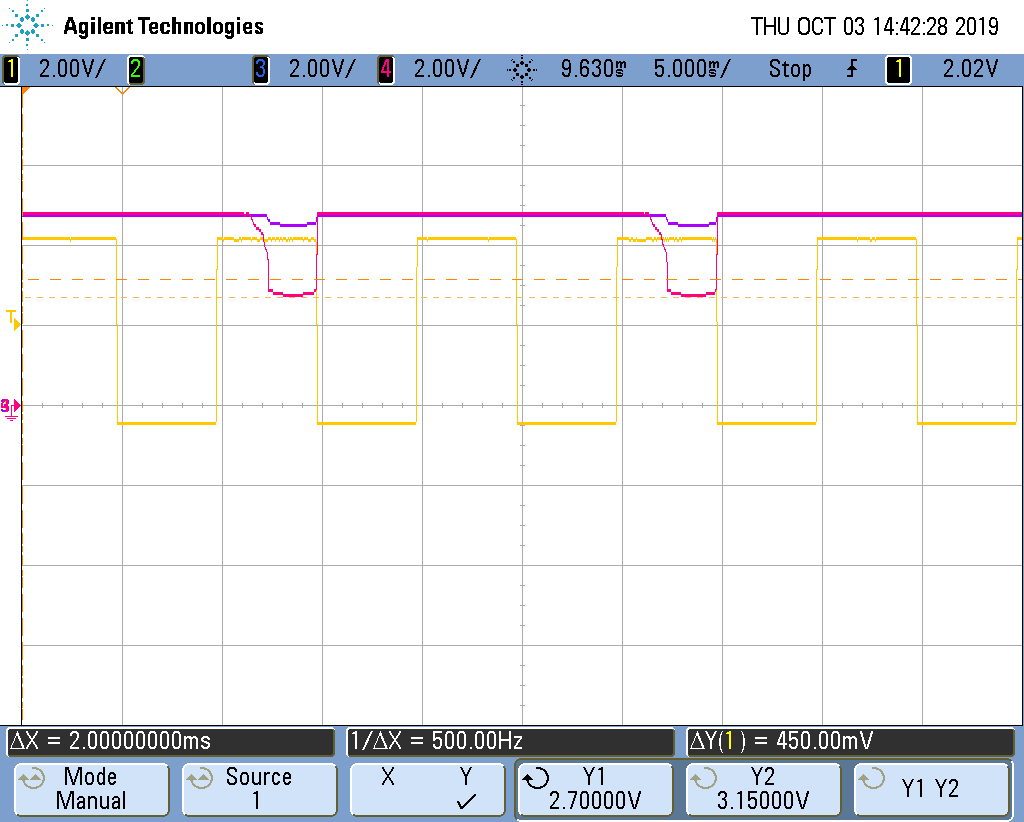
\includegraphics[width=0.8\textwidth, trim = {0 0 0 2cm},clip]{ImagenesEjercicio3/scope_5.png}
	\caption{Salida con glitch (rosa) y sin glitch (violeta) variando $b$ (amarillo).}
	\label{fig:medicion}
\end{figure}

Se observa de la figura anterior como la salida varía en función de la entrada. Si bien la señal que no posee la solución al glitch (señal rosada) no decae por completo a un cero lógico, esta posee una variación importante, la cual vale destacar. Dicha variación coloca la tensión a la salida de la primer compuerta OR por debajo de los $3.15 \ V$, valor que, según la tecnología adoptada, es menor a la tensión $V_{OH}$, por ende, este valor deja de ser considerado como un uno lógico. Por un lado, se denota que la señal que sí posee dicha solución (señal violeta) también posee una variación, la cual no es de importancia ya que se sigue manteniendo dentro del rango $V_{IH} \sim Vcc$, de forma el valor lógico de esta salida no varía.

\end{document}
\newpage
\section{Ejercicio 4}
%	\input{../Ejercicio 4/Ejercicio 4.tex}
\newpage	
\section{Ejercicio 5}
%	\documentclass[a4paper]{article}
\usepackage[utf8]{inputenc}
\usepackage[spanish, es-tabla]{babel}
\usepackage[table,xcdraw]{xcolor}
\usepackage{amsmath}
\usepackage{amsfonts}
\usepackage{amssymb}

\usepackage{float}
\usepackage{graphicx}

\usepackage{caption}
\usepackage{subcaption}
\captionsetup{compatibility=false}

\usepackage{multirow}
\setlength{\doublerulesep}{\arrayrulewidth}

\newcommand{\quotes}[1]{``#1''}
\newcommand\underrel[2]{\mathrel{\mathop{#2}\limits_{#1}}}

\usepackage{array}
\newcolumntype{C}[1]{>{\centering\let\newline\\\arraybackslash\hspace{0pt}}m{#1}}

\usepackage[american]{circuitikz}
\usepackage{xcolor}
\usepackage{fancyhdr}

\newlength{\stockheight}
\usepackage{hyperref}

\hypersetup{
    colorlinks=true,
    linkcolor=blue,
    filecolor=magenta,      
    urlcolor=blue,
    citecolor=blue,    
}

\urlstyle{same}

\usepackage{units} 
\pagestyle{fancy}
\fancyhf{}

\rfoot{Página \thepage}

\begin{document}
\subsection{Introducción}
En esta sección se procedio a realizar el analisis de dos compuertas lógicas de distintas tecnologías que consisten en una compuerta \textbf{AND} de tecnología TTL y una compuerta \textbf{OR} CMOS conectadas de la siguiente forma

\subsection{Análisis compuerta AND open gate}
Para realizar este análisis se utilizó una de las 4 compuertas que brinda el integrado SN74S08, como es una compuerta AND y una de sus entradas ya esta conectada a $ V_CC $ la señal de salida dependerá solo del valor que tenga la señal en esa sola entrada. Ahora dejando al vacio esa entrada se puede observar que el valor que se obtiene a la salida corresponde a HIGH(1 lógico), esto ocurre debido se esta dejando al vacio el emisor del transistor al que le corresponde esa entrada por lo tanto dicho transistor se encuentra al corte lo que hace que a la salida siempre se vea HIGH.

\subsection{Análisis compuerta OR open gate}
En este caso se utiizó una de las compuertas lógicas que brinda el integrado CD4071 pero en este caso se conecto uno de sus pines de entrada a $ GND $ y se dejó otro abierto. En este caso el valor que se ve a la salida también solo depende del valor de la entrada que se dejó abierta. Como la alta impedencia de

\subsection{Análisis ambas compuertas conectadas entre si}
Utilizando los circuitos ahora se los conecto de la siguienta manera:
\begin{figure}[h]
    \centering
    
\includegraphics{Imagenes/pend.jpg}
    \caption{Conexión de la AND con la OR}
\end{figure}

La salida de este circuito por lo analizado en los puntos anteriores solo depende de la señal de entrada que se va a utilizar. Analizando las hojas de datos de ambos integrados y utilizando una alimentación $V_{DD}= 4.5V $ se obtiene que la tensión mínima de la salida en estado alto es $V_{OH}=2.5 V$ que cae en el rango de valores indeterminados para la OR cuya $V_{IL}= 3.15 V$ en el peor de los casos, lo que puede ocasionar que a pesar de que la salida de la AND sea HIGH a la salida total del circuito se vea un LOW o 0.


\subsection{Solución al problema anterior}

Una solución al problema mencionado anteriormente es utilizar un circuito llamado level shifter que se puede fabricar utilizando un transistor PNP y un par de resistencias. Este circuito tomará la salida de la primer compuerta y en el caso de que está fuera HIGH llevará dicho valor a un nivel de tensión mas alto para que así la compuerta siguiente pueda tomar correctamente el valor que debería recibir.


\begin{figure}[h]
    \centering
    
\includegraphics{Imagenes/pend.jpg}
    \caption{Implementación del level shifter}
\end{figure}


\end{document}
\newpage
\section{Ejercicio 6}
	
%\documentclass[a4paper]{article}
\usepackage[utf8]{inputenc}
\usepackage[spanish, es-tabla]{babel}

\usepackage[a4paper, footnotesep = 1cm, width=18cm, left=2cm, top=2.5cm, height=25cm, textwidth=18cm, textheight=25cm]{geometry}
%\geometry{showframe}

\usepackage{tikz}
\usepackage{amsmath}
\usepackage{amsfonts}
\usepackage{amssymb}
\usepackage{float}
\usepackage{graphicx}
\usepackage{caption}
\usepackage{subcaption}
\usepackage{multicol}
\usepackage{multirow}
\setlength{\doublerulesep}{\arrayrulewidth}
\usepackage{xcolor}

\usepackage{hyperref}
\hypersetup{
    colorlinks=true,
    linkcolor=blue,
    filecolor=magenta,      
    urlcolor=blue,
    citecolor=blue,    
}

\newcommand{\quotes}[1]{``#1''}
\usepackage{array}
\newcolumntype{C}[1]{>{\centering\let\newline\\\arraybackslash\hspace{0pt}}m{#1}}
\usepackage[american]{circuitikz}
\usepackage{fancyhdr}
\usepackage{units} 

\pagestyle{fancy}
\fancyhf{}
\lhead{22.13 Electrónica III}
\rhead{Mechoulam, Lambertucci, Martorell, Londero}
\rfoot{\center \thepage}




Es esta sección se implementará un SR-Latch y un Flip Flop D utilizando compuertas.
\subsection{SR-Latch}
Un Latch-SR es un elemento de memoria asincrónico, con dos inputs (S-R) también conocido con Set-Reset Latch. Le corresponde la siguiente tabla de verdad:

\begin{table}[H]
\centering
\begin{tabular}{
>{\columncolor[HTML]{FFFFFF}}c 
>{\columncolor[HTML]{FFFFFF}}c |
>{\columncolor[HTML]{FFFFFF}}c }
\textbf{$S$} & \textbf{$R$} & \textbf{$Q_n$} \\ \hline
0            & 0            & $Q_{n-1}$      \\
0            & 1            & 0              \\
1            & 0            & 1              \\
1            & 1            & 0             
\end{tabular}
\end{table}
Se propucieron dos circuitos de implementación siendo uno implementado con NOR y uno con NAND con la intención de no solo comparar los observables de interes con un modelo comercial sino tambien entre distintas tipos de compuertas.Siendo los siguientes circuitos:\footnote{Brown, S. and Vranesic, Z. (2002). Fundamentals of digital logic with VHDL design. 3rd ed. pp.250-251.}:
\begin{figure}[H]	
	\centering
	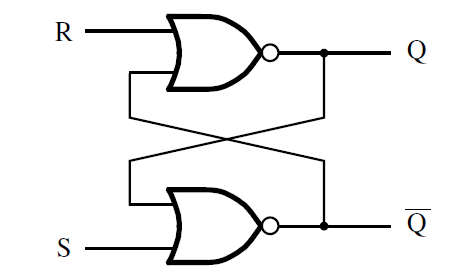
\includegraphics[width=0.4\textwidth]{Imagenes/srlatch.PNG}
	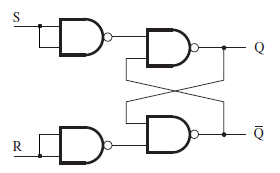
\includegraphics[width=0.4\textwidth]{Imagenes/LATCHNAND.PNG}
	\caption{Circuito Propuesto SR-Latch.}
	\label{fig:circsrlatch}
\end{figure}
Se llevará a cabo utilizando compuertas NOR y NAND, se eligió el integrado \href{https://pdf1.alldatasheet.com/datasheet-pdf/view/228632/ONSEMI/74HC02.html}{74HC02} debido a que es High-Speed y no es necesario compatibilidad con TTL, como se analizó en el punto (2). 

Se tomarán como observables  de interés el tiempo de propagación:
\begin{align} t_{p-SQ}: S \implies Q \ \ \ \textsuperscript{$\wedge$} \ \ \ t_{p-RQ}: R \implies Q \end{align} 

Estos tiempos serán comparados con un integrado \href{http://noel.feld.cvut.cz/hw/st/1937.pdf}{74HC279} el cual contiene 4 SR-Latch.

Las mediciones hechas se ven en la siguiente tabla:
\begin{table}[H]
\centering
\begin{tabular}{cccl}
\textit{}           & \textbf{Circuito NOR} & \textbf{Circuito NAND} & \textbf{74HC279} \\ \hline
\textbf{$t_{p-RQ}$} & 8.3nS                 & 43.2ns                 & 8nS              \\
\textbf{$t_{t-RQ}$} & 4.83nS                & 4nS                    & 14nS             \\
\textbf{$t_{p-SQ}$} & 24.24nS               & 18ns                   & 15nS             \\
\textbf{$t_{t-SQ}$} & 11nS                  & 4ns                    & 8nS             
\end{tabular}
\end{table}
Es notable que los tiempos son bastante similares, el espacio que ocupan no lo es, dado que toma el doble de integrados para la misma cantidad de Latches. 
\subsection{Flip Flop D}
Un Flip Flop D es un elemento de memoria sincrónico,cuenta con  2 entradas siendo una de clock y la otra de la información (Data).Le corresponde la siguiente tabla de verdad:
% Please add the following required packages to your document preamble:
% \usepackage[table,xcdraw]{xcolor}
% If you use beamer only pass "xcolor=table" option, i.e. \documentclass[xcolor=table]{beamer}
\begin{table}[H]
\centering
\begin{tabular}{
>{\columncolor[HTML]{FFFFFF}}c 
>{\columncolor[HTML]{FFFFFF}}c |
>{\columncolor[HTML]{FFFFFF}}c }
\textbf{Clock} & \textbf{$D$} & \textbf{$Q_n$} \\ \hline
$\downarrow$   & X            & $Q_{n-1}$      \\
$\uparrow$     & 0            & 0              \\
$\uparrow$     & 1            & 1             
\end{tabular}
\end{table}
El circuito propuesto de implementación es el siguiente:\footnote{Brown, S. and Vranesic, Z. (2002). Fundamentals of digital logic with VHDL design. 3rd ed. pp.254-256.}:
\begin{figure}[H]	
	\centering
	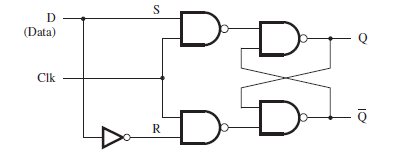
\includegraphics[width=0.8\textwidth]{Imagenes/dff.PNG}
	\caption{Circuito Propuesto Flip Flop D.}
	\label{fig:circsrlatch}
\end{figure}
Se llevará a cabo utilizando compuertas NAND, se eligió el integrado \href{https://pdf1.alldatasheet.com/datasheet-pdf/view/351460/ONSEMI/74HC132.html}{74HC132}  debido a que es High-Speed y no es necesario compatibilidad con TTL, como se analizó en el punto (2). 
También para el clock se realizó un edge-Detector implementado con el siguiente circuito:
\begin{figure}[H]	
	\centering
	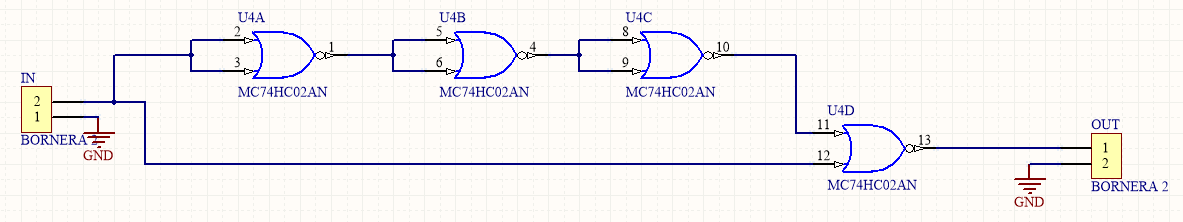
\includegraphics[width=0.8\textwidth]{Imagenes/edgedetector.PNG}
	\caption{Edge detector.}
	\label{fig:circedge}
\end{figure}
El cual es anexado al circuito implementado con NANDS del latch SR.


Se tomarán como observables  de interés el tiempo de propagación y de transición:
\begin{align} t_{p-DQ}: D \implies Q \ \ \ t_{t-DQ}: Q=0 \implies Q = 1 \end{align} 
En cuanto a la medición de estos tiempos, se tuvo la problemática de que el rise time de las compuertas eran menores que el rise time del osciloscopio, en algunas de ellas se logró conseguir un osciloscopio con mayor ancho de banda lo cual mejoró las mediciones.

Estos tiempos medidos serán comparados con un integrado \href{https://pdf1.alldatasheet.com/datasheet-pdf/view/15593/PHILIPS/74HC374.html}{74HC374} el cual contiene 8 Flip Flop D.
Las mediciones hechas se ven en la siguiente tabla:
\begin{table}[H]
\centering
\begin{tabular}{ccc}
\textit{}                               & \textbf{Circuito}         & \textbf{74HC374}     \\ \hline
\textbf{$t_{p-DQ}$}                     & 23.6nS                    & 16nS                 \\
\textbf{$t_{t-DQ}$}                     & 4.43nS                    & 5nS                  \\
\end{tabular}
\end{table}


\newpage
\section{Ejercicio 7}
%	%%%%%%%%%%%%%%%%%%%%%%%%%BORRAR
\documentclass[a4paper]{article}
\usepackage[utf8]{inputenc}
\usepackage[spanish, es-tabla]{babel}

\usepackage[a4paper, footnotesep = 1cm, width=18cm, left=2cm, top=2.5cm, height=25cm, textwidth=18cm, textheight=25cm]{geometry}
%\geometry{showframe}

\usepackage{tikz}
\usepackage{amsmath}
\usepackage{amsfonts}
\usepackage{amssymb}
\usepackage{float}
\usepackage{graphicx}
\usepackage{caption}
\usepackage{subcaption}
\usepackage{multicol}
\usepackage{multirow}
\setlength{\doublerulesep}{\arrayrulewidth}
\usepackage{xcolor}

\usepackage{hyperref}
\hypersetup{
    colorlinks=true,
    linkcolor=blue,
    filecolor=magenta,      
    urlcolor=blue,
    citecolor=blue,    
}

\newcommand{\quotes}[1]{``#1''}
\usepackage{array}
\newcolumntype{C}[1]{>{\centering\let\newline\\\arraybackslash\hspace{0pt}}m{#1}}
\usepackage[american]{circuitikz}
\usepackage{fancyhdr}
\usepackage{units} 

\pagestyle{fancy}
\fancyhf{}
\lhead{22.13 Electrónica III}
\rhead{Mechoulam, Lambertucci, Martorell, Londero}
\rfoot{\center \thepage}
\begin{document}
\section{auxiliar}
\tableofcontents
%%%%%%%%%%%%%%%%%%%%%%%%%BORRAR

\subsection{Introducción}
\subsubsection{Contadores}
		Los contadores son dispositivos digitales capaces de almacenar la cantidad de pulsos que este recibe. Como todo almacenamiento digital requiere de memoria, los contadores están generalmente constituidos por varias celdas de almacenamiento de 1 bit, comúnmente usados los JK flip-flops. Se puede contemplar la implementación de un JK flip-flip en la Figura (\ref{circ:fkflipflop}) utilizando solamente compuertas lógicas discretas. 
		
		\begin{figure}[H]
	\hspace*{-1cm}
	\centering
	\scalebox{0.7}{
	\begin{circuitikz}
		\draw	
	
			%%%%%%%%%%%%%%%%%%%%%%%%%%%%%
			%FIGURAS
			%%%%%%%%%%%%%%%%%%%%%%%%%%%%%
			
			node[nor port](nor1){} %NOR1
				to[open] ++ (0, -2)
			node[nor port](nor2){} %NOR2
			
			(nor1.in 1) to[open] ++ (-2, 0)
			node[and port, number inputs = 3](and1){} %AND1
			
			(nor2.in 2) to[open] ++ (-2, 0)
			node[and port, number inputs = 3](and2){} %AND2
			
			%%%%%%%%%%%%%%%%%%%%%%%%%%%%%	
	
			(nor1.out) to[short, -*] ++ (0.5, 0)
					node[](feedback1){}
				to[short] ++ (0.5, 0)
				to[short, -*] ++ (0.5, 0)
					node[](feedback2){}
				to[short, -o] ++ (0.5, 0)
				node[label=east:$Q$]{}
			
			(nor2.out) to[short, -*] ++ (0.5, 0)
					node[](feedback3){}
				to[short, -*] ++ (0.5, 0)
					node[](feedback4){}
				to[short] ++ (0.5, 0)
				to[short, -o] ++ (0.5, 0)
				node[label=east:$\overline{Q}$]{}
				
			(feedback1) to[short] ++ (0, -0.38)
				to[short] ++ (-3, -1)
				to[short] ++ (0, -0.3)
				|- (nor2.in 1)
				
			(feedback3) to[short] ++ (0, 0.38)
				to[short] ++ (-3, 1)
				to[short] ++ (0, 0.3)
				|- (nor1.in 2)
				
			(nor1.in 1) -- (and1.out)
			(nor2.in 2) -- (and2.out)
			
			(and1.in 2) to[short, -o] ++ (-1, 0)
				node[label=west:$J$]{}
			
			(and2.in 2) to[short, -o] ++ (-1, 0)
				node[label=west:$K$]{}
				
			(and1.in 3) to[short] ++ (-0.5, 0)
				to[short, -*] ++ (0, -0.922)
				node[](enable){}
				|- (and2.in 1)
				
			(and2.in 3)	to[short] ++ (-0.5, 0)
				|- ++ (6, -0.5)
				-| (feedback2.center)
				
			(and1.in 1) to[short] ++ (-0.5, 0)
				|- ++ (5.5, 0.6)
				-| (feedback4.center)
				
			(enable) to[short] ++ (-0.5, 0)
				to[twoport, -o, l_=Edge Det] ++ (-3, 0)
				node[label=west:$CLK$]{}
	
		;
	\end{circuitikz}
	}
	\caption{Implementación de un JK flip-flop con una totalidad de 8 compuertas lógicas discretas (teniendo en cuenta la implementación de las compuertas AND de tres entradas junto a la corrección de delay.}
	\label{circ:fkflipflop}
\end{figure}
		
		La cantidad de flip-flops necesaria para construir un contador está ligada al mayor número que el dispositivo puede almacenar. Si se quiere contar hasta el número $N$, el contador tendrá que disponer como mínimo de $\lceil log_2(N) \rceil$ flip-flops. Existen dos tipos de contadores: asíncronos y síncronos.
		
\subsubsection{Contadores Asíncronos}
		Los contadores asíncronos poseen un único flip-flop cuya entrada esté conectada al generador de pulsos, propagándose la información provista por este a través del resto para aumentar el contador. Es por esta razón que a los contadores asíncronos se los suele denominar también como contadores por propagación o \textit{ripple counters} en inglés. 

\begin{figure}[H]
	\centering
	\begin{circuitikz}
		\draw
			node[ocirc, label=west:$CLK$]{}
				to[short] ++ (1, 0)
				to[open] ++ (2, 1)
				node[fourport](1){}
				to[open] ++ (3, 0)
				node[fourport](2){}
				to[open] ++ (3, 0)
				node[fourport](3){}
				to[open] ++ (3, 0)
				node[fourport](4){}
				to[open] ++ (-11, -1)
				|- (1.1)
				(1.2) -- (2.1)
				(2.2) -- (3.1)
				(3.2) -- (4.1)
				
				(1.1) ++ (0.13,0) node[]{\scalebox{1.2}{\rotatebox{-90}{$\triangle$}}}
				(2.1) ++ (0.13,0) node[]{\scalebox{1.2}{\rotatebox{-90}{$\triangle$}}}
				(3.1) ++ (0.13,0) node[]{\scalebox{1.2}{\rotatebox{-90}{$\triangle$}}}
				(4.1) ++ (0.13,0) node[]{\scalebox{1.2}{\rotatebox{-90}{$\triangle$}}}
		;
	\end{circuitikz}
	\caption{Conección entre flip-flops para un contador asíncrono.}
	\label{circ:async_counter_connection}		
\end{figure}				
		
		Como los pulsos deben de propagarse a lo largo de varias compuertas lógicas, sucede que para cada incremento en el contador, no todos los bits de la palabra almacenada cambian al mismo instante. En la Figura (\ref{async_ripple}) se esquematiza este efecto para un contador que transita de almacenar un $0111_2$ a almacenar un $1000_2$.

\begin{figure}[H]
	\centering
	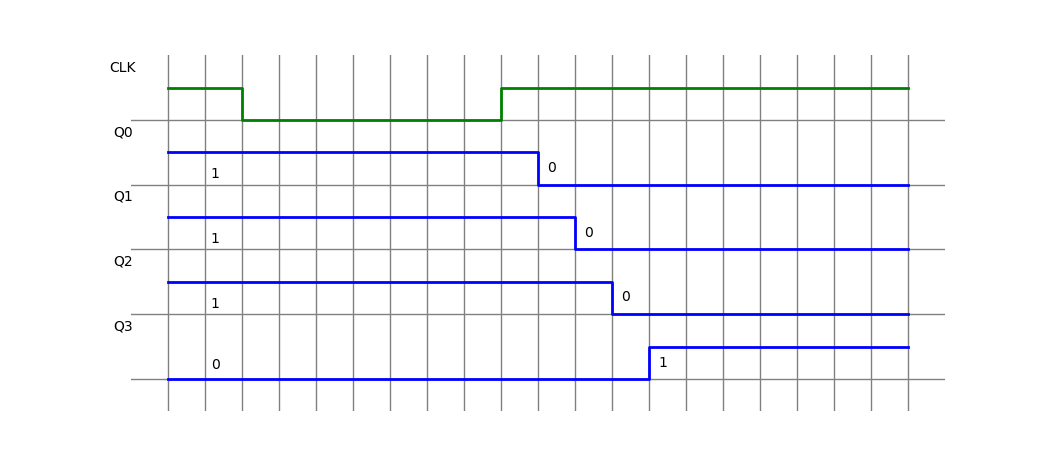
\includegraphics[width=0.7\textwidth]{Imagenes/async_ripple.png}
	\caption{Propagación de un pulso recibido a través de un contador asíncrono para la palabra almacenada transitando del estado $(7)_{10}$ al estado $(8)_{10}$.}
	\label{async_ripple}
\end{figure}

Debido a este fenómeno, las implementaciones asíncronas de contadores no son del todo fidedignas. Sin embargo, abundan como divisores de frecuencia ya que la salida de cada flip-flop será la frecuencia de los pulsos de entrada dividida por una potencia de dos. Otra desventaja de los contadores asíncronos está directamente relacionada con la anterior y es que debido al fenómeno de propagación estos dispositivos se vuelven mucho más lentos en comparación a otros tipos de contadores.

No obstante, la ventaja de esta implementación es que estos dispositivos son muy simples y fáciles de contruir.

\subsubsection{Contadores Síncronos}

\begin{figure}[H]
	\centering
	\begin{circuitikz}
		\draw
			node[ocirc, label=west:$CLK$]{}
				to[short] ++ (1, 0)
					node[](hola){}
				to[open] ++ (2, 1.5)
				node[fourport](1){}
				to[open] ++ (3, 0)
				node[fourport](2){}
				to[open] ++ (3, 0)
				node[fourport](3){}
				to[open] ++ (3, 0)
				node[fourport](4){}
				to[open] ++ (-11, -1)

				(1.1) to[short] ++ (-0.5,0)
					to[short, -*] ++ (0, -1.05)
				(2.1) to[short] ++ (-0.5,0)
					to[short, -*] ++ (0, -1.05)
				(3.1) to[short] ++ (-0.5,0)
					to[short, -*] ++ (0, -1.05)
				(4.1) to[short] ++ (-0.5,0)
					to[short] ++ (0, -1.05)
					to[short] (hola)
				
				
				
				(1.1) ++ (0.13,0) node[]{\scalebox{1.2}{\rotatebox{-90}{$\triangle$}}}
				(2.1) ++ (0.13,0) node[]{\scalebox{1.2}{\rotatebox{-90}{$\triangle$}}}
				(3.1) ++ (0.13,0) node[]{\scalebox{1.2}{\rotatebox{-90}{$\triangle$}}}
				(4.1) ++ (0.13,0) node[]{\scalebox{1.2}{\rotatebox{-90}{$\triangle$}}}
		;
	\end{circuitikz}
	\caption{Conección entre flip-flops para un contador síncrono.}
	\label{circ:sync_counter_connection}		
\end{figure}	

\end{document}
\newpage
\section{Ejercicio 8}
%	%%%%%%%%%%%%%%%%%%%%%%%%%BORRAR
\documentclass[a4paper]{article}
\usepackage[utf8]{inputenc}
\usepackage[spanish, es-tabla]{babel}

\usepackage[a4paper, footnotesep = 1cm, width=18cm, left=2cm, top=2.5cm, height=25cm, textwidth=18cm, textheight=25cm]{geometry}
%\geometry{showframe}

\usepackage{tikz}
\usepackage{amsmath}
\usepackage{amsfonts}
\usepackage{amssymb}
\usepackage{float}
\usepackage{graphicx}
\usepackage{caption}
\usepackage{subcaption}
\usepackage{multicol}
\usepackage{multirow}
\setlength{\doublerulesep}{\arrayrulewidth}
\usepackage{xcolor}

\usepackage{hyperref}
\hypersetup{
    colorlinks=true,
    linkcolor=blue,
    filecolor=magenta,      
    urlcolor=blue,
    citecolor=blue,    
}

\newcommand{\quotes}[1]{``#1''}
\usepackage{array}
\newcolumntype{C}[1]{>{\centering\let\newline\\\arraybackslash\hspace{0pt}}m{#1}}
\usepackage[american]{circuitikz}
\usepackage{fancyhdr}
\usepackage{units} 

\pagestyle{fancy}
\fancyhf{}
\lhead{22.13 Electrónica III}
\rhead{Mechoulam, Lambertucci, Martorell, Londero}
\rfoot{\center \thepage}
\begin{document}
\section{auxiliar}
\tableofcontents
%%%%%%%%%%%%%%%%%%%%%%%%%BORRAR

\subsection{Introducción}

Los mandos de control o actualmente llamados \quotes{Joysticks} son parte fundamental de varios dispositivos electrónicos utilizados hoy en día. Consolas de videojuegos, sillas de ruedas eléctricas, aeronaves radio-controladas e incluso hasta cohetes de la NASA. En su forma más básica, un potenciómetro, los mandos de control revolucionaron al rededor de finales de la segunda guerra mundial la manera de controlar dispositivos digitales de manera analógica. 

En esta sección del informe nos centraremos en la implementación de un convertidor analógico a digital mediante el uso del Joystick HW-504 junto a la investigación realizada.

\subsection{Joystick HW-504}

\begin{figure}[H]
	\centering
	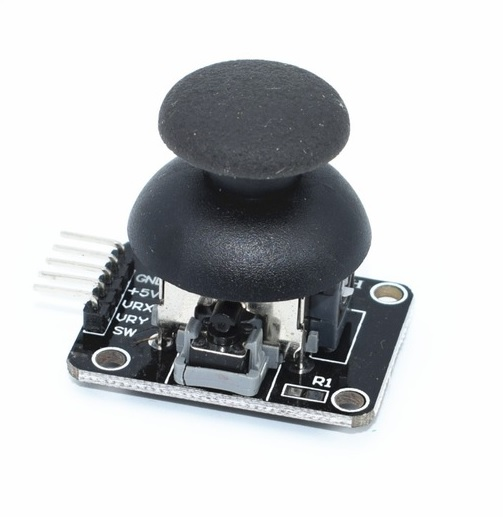
\includegraphics[width=0.5\textwidth]{Imagenes/joystick.jpg}
	\caption{Mando de control HW-504 a utilizar.[1]}
	\label{fig:joystick}
\end{figure}

El mando de control a utilizar está compuesto por dos potenciómetros, uno para el eje X y otro para el eje Y, y un switch accionado al apretar el mando hacia dentro. El periférico requiere de una alimentación de $5V$ y puede esquematizarse como el siguiente modelo electóonico:

\begin{figure}[H]
\centering
\begin{circuitikz}

\draw

(0,0) node[label=west:{\color{blue}\textbf{+5V}}](5V){}
	to[short,o-*] ++ (2, 0)
	node[](LEFT_POTX_NODE){}
	
(LEFT_POTX_NODE) to[pR, -*, name=pot-x] ++ (5, 0)
	node[](RIGHT_POTX_NODE){}

(pot-x.wiper) to[short, -o] ++ (0, 0)
	node[label=north:{\color{blue}\textbf{VRx}}](){}

(LEFT_POTX_NODE) to[short, -*] ++ (0, -2)
	node[](LEFT_POTY_NODE){}
	to[pR, -*, name=pot-y] ++ (5, 0)
	
(pot-y.wiper) to[short, -o] ++ (0,0)
	node[label=north:{\color{blue}\textbf{VRy}}](){}
	
(LEFT_POTY_NODE) to[short] ++ (0, -1.7)
	node[](LEFT_SW_NODE){}
	to[push button] ++ (5, 0)
	to[short, -o] ++ (2,0)
	node[label=east:{\color{blue}\textbf{SW}}](SW){}
	
(RIGHT_POTX_NODE) to[short] ++ (0, -2)

(RIGHT_POTX_NODE) to[short, -o] ++ (2, 0)
	
	node[label=east:{\color{blue}\textbf{GND}}]{}

;

\end{circuitikz}
\caption{Circuito equivalente del mando HW-504 con mismos nombres que el pin-out del periférico.}
\label{circuit:joytick_eq}
\end{figure}

\subsection{Bibliografía}
[1]Eshop.tecnoconciencia.com.ve, 2019. [Online]. Available: https://eshop.tecnoconciencia.com.ve/eshop/wp-content/uploads/2017/08/JOYSTICK-ARDUINO.jpg. [Accessed: 23- Sep- 2019].

\end{document}

\end{document}